\documentclass[12pt,a4paper]{article}

% === Encoding and fonts ===
\usepackage[utf8]{inputenc}
\usepackage[T1]{fontenc}
\usepackage{mathpazo}
\usepackage{amsmath}

% === Page layout ===
\usepackage{geometry}
\geometry{margin=2.5cm}

% === Typography and spacing ===
\usepackage{microtype}
\usepackage{parskip}
\usepackage{needspace}
\setlength{\emergencystretch}{2em}
\clubpenalty=10000
\widowpenalty=10000
\displaywidowpenalty=10000
\brokenpenalty=10000
\interfootnotelinepenalty=10000
\raggedbottom
\usepackage{setspace}
\onehalfspacing

% === Tables and figures ===
\usepackage{booktabs}
\usepackage{graphicx}
\graphicspath{{figures/}}
\usepackage{float}
\usepackage{longtable}
\usepackage{array}
\usepackage{caption}
\captionsetup{font={small,stretch=1.0},labelfont=bf,skip=6pt}

% Floats may use b and p as well as h and t; placeins stops floats crossing sections.
\usepackage[section]{placeins}
\renewcommand{\topfraction}{0.9}
\renewcommand{\bottomfraction}{0.7}
\renewcommand{\textfraction}{0.1}
\renewcommand{\floatpagefraction}{0.7}
\setcounter{topnumber}{3}
\setcounter{bottomnumber}{2}
\setcounter{totalnumber}{5}

% === Citations: Harvard style (natbib + agsm) ===
\usepackage{natbib}
\bibliographystyle{agsm}
\setcitestyle{authoryear,open={(},close={)}}

% === Hyperlinks and URL-safe bibliography links ===
% agsm.bst emits \harvardurl{...}; without this, underscores in URLs break compilation.
\usepackage{xurl}
\usepackage[colorlinks=true,linkcolor=blue!60!black,citecolor=blue!60!black,urlcolor=blue!60!black]{hyperref}
% \url must read the URL itself (no #1 argument), or a % in a URL (e.g. %20) starts a comment and breaks the bibliography.
\renewcommand{\harvardurl}{\textbf{URL:} \url}
\usepackage{pdfpages}
\usepackage[dvipsnames]{xcolor}
\urlstyle{same}
% xurl's break list without the full stop, so a URL never breaks straight after "." (e.g. before "zip").
\def\UrlBreaks{\do\@\do\\\do\/\do\!\do\_\do\|\do\;\do\>\do\]%
\do\)\do\,\do\?\do\&\do\'\do+\do\=\do\#\do:%
\do\a\do\b\do\c\do\d\do\e\do\f\do\g\do\h\do\i\do\j\do\k\do\l%
\do\m\do\n\do\o\do\p\do\q\do\r\do\s\do\t\do\u\do\v\do\w\do\x\do\y\do\z%
\do\A\do\B\do\C\do\D\do\E\do\F\do\G\do\H\do\I\do\J\do\K\do\L%
\do\M\do\N\do\O\do\P\do\Q\do\R\do\S\do\T\do\U\do\V\do\W\do\X\do\Y\do\Z%
\do0\do1\do2\do3\do4\do5\do6\do7\do8\do9}
\setlength{\bibsep}{6pt plus 1pt minus 1pt}
\makeatletter
\setlength{\@fptop}{0pt}
\makeatother

% ============================================================================

\begin{document}
% The unnumbered title must not duplicate the abstract's page.1 destination.
\hypersetup{pageanchor=false}

\begin{titlepage}
\centering
\vspace*{1cm}

\includegraphics[width=4cm]{uct_logo.jpg}\\[1cm]
{\Large University of Cape Town\\[0.3cm]}
{\large School of Economics\\[0.3cm]}
{\large ECO5016W FinTech Mini-Dissertation\\[2cm]}

{\LARGE\bfseries Who Writes the Token Ledger?\\[0.4cm]
\large Holders, Transfer Agents and\\[0.15cm] Four Tokenised U.S. Money Market Funds\\[2cm]}

{\large Karabo Tigedi\\[0.3cm]}
{\large TGDMOE001\\[0.3cm]}
{\large Supervisor: Dr Allan Davids\\[2cm]}

\vfill
{\small Word count: 5949} % set from: python scripts/submission_wordcount.py (confirmed exclusions; figure caption included)
\end{titlepage}
\hypersetup{pageanchor=true}

% Signed AI/plagiarism declarations and Turnitin report are uploaded separately
% on Amathuba, as confirmed by the student on 15 November 2026.

\newpage
\begin{abstract}
\noindent Tokenisation is said to remove the layers between investors and assets, making settlement immediate, servicing automatic and minimums small. I test that claim on the four tokenised United States government money market funds that report monthly to the Securities and Exchange Commission, offered by Franklin Templeton, WisdomTree, JPMorgan and Fidelity, and ask what South Africa should do. The evidence combines up to 28 monthly filings per fund, public blockchain records frozen in October 2026, transfer signatures and prospectuses.

Three roles turn out to be separable: appearing as a party to a transfer, authorising it, and making the entry that counts in law as ownership. Franklin and WisdomTree divide them in opposite ways. Franklin's blockchain is part of its official ownership record, but every observed holder-to-holder transfer was signed with keys that are, or were, signers on the issuer's own account. WisdomTree's holders sign their own transfers (most of the value involving one wallet matched to its parent company), but a transfer is valid only once the transfer agent records it off chain. WisdomTree's tokens match its filed shares exactly, with no adjustment, in all ten months that could be checked; the match depends on a choice, made after the calibration window, not to count dividend tokens minted the next morning; counting them would open small gaps in six months.

The economic change is narrow. Issuance and redemption still follow bank business days; WisdomTree's two exchange routes through contracts, mostly atomic, carry volume equal to 2.9\% of its gross redemptions; and Fidelity's on-chain class yields two basis points less than an otherwise identical untokenised class, a price for the class rather than a measured cost of the technology.

For South Africa, I recommend a technology-neutral reading of existing law now, a conditional pilot under existing powers, and a narrow clarification of the draft exchange-control rules, not a broad security-token definition, because the binding questions are which record governs and who writes it. The evidence is descriptive and covers four young funds.
\end{abstract}

\newpage
\begin{singlespace}
\tableofcontents
\end{singlespace}
\newpage

\section{Introduction}\label{sec:intro}
Tokenisation promises to put the ownership record, the terms of a claim and the payment on one shared ledger, so that settlement is immediate, servicing automatic and minimum investments small, with fewer intermediaries in between. Tokenised government money market funds are a natural test: their portfolios are already liquid and electronic, so if a token ledger can take over intermediaries' record-keeping anywhere, it should be here.

Testing it requires keeping three roles apart. A holder can appear in a token transfer as sender or recipient. Someone authorises the transfer by signing it. And someone makes the entry that counts in law as ownership. The first two can move to holders without the third moving with them, so token activity alone cannot show that an intermediary has been replaced.

The research question is: \textit{When U.S. government money market funds record their shares on public blockchains, does the token ledger take over any function of the transfer agent and the intermediaries around it (keeping the record, settling issuance and redemption, servicing distributions, holding for investors), or does it follow records those intermediaries have already made? What does South African law currently provide for each of these functions, and which route should South Africa take: a security-token definition, a pilot regime, or a technology-neutral reading of existing law?}

The answer differs by function, and the clearest contrast is between Franklin Templeton and WisdomTree. At Franklin the chain counts in law under the fund's own prospectus, which makes the blockchain part of its official ownership record, but holders do not sign their transfers: every observed holder-to-holder transfer was signed with keys that are, or were, also signers on the issuer's own account. At WisdomTree holders do sign (though most holder-to-holder value involves one wallet matched to the sponsor's parent company), but the chain does not count in law: a transfer is valid only once the transfer agent registers it in an off-chain book. Neither fund gives the holder both the signature and the legally effective entry. The economic change is narrow: issuance and redemption keep bank business days, the exchange routes through contracts are small, and Fidelity's two-basis-point class difference is a price set for the class, not a measured cost of the blockchain.
% src: prep_permissions_matrix.csv items i--ii (FOBXX p.6; WTGXX p.143); key_numbers.csv addl_signer_n__FOBXX__stellar__issuer_account_signer_keys_current_or_former_sign = 44; addl_pmwallet_f1_lower_value_touching_share_of_lower_pct = 99.6879; addl_contract_venue_ratio.csv; exploratory/2026-11-17/fidelity_class_gap_summary.csv (paired 2026 gap -0.0199)

For South Africa I argue for three things: a technology-neutral reading of existing law now, a conditional pilot under existing regulatory powers, and an immediate, narrow clarification of the draft exchange-control instruments, which on their wording would treat a tokenised fund unit as a crypto asset. A broad security-token definition would not settle what the four funds show to be binding: which record governs, who may write to it and how the cash leg, the payment side of each trade, settles.

The contribution is to set filings, chain records, signatures and prospectus terms side by side for the four funds of this kind identified in the regulator's monthly filings, so that each role is traced separately rather than inferred from token activity. Sections~\ref{sec:lit} and~\ref{sec:method} set out the claims and the data, Sections~\ref{sec:m0} to~\ref{sec:econ} the results and their economics, Sections~\ref{sec:sa} and~\ref{sec:policy} South African law and policy, and Section~\ref{sec:limits} the limits.

\section{What tokenisation is claimed to change}\label{sec:lit}
What is tokenised here is the fund share, not the portfolio \citep[p.~10]{FSB2024}, and blockchain records play different legal roles across products \citep[pp.~10, 46, 64]{IOSCO2025}. The literature ties each claimed benefit to a condition.

The first claim is faster settlement. In \citet[pp.~31, 42]{ChiuKoeppl2019}, the gain shrinks as legacy settlement approaches immediacy, and delivery versus payment requires the asset and the payment to be linked. \citet[pp.~130--131]{BenosGarrattGurrolaPerez2019} add that representing an off-ledger asset may need a trusted guarantor that tokens and assets correspond. The FSB accepts settlement assets on a fully interoperable platform but stresses links to infrastructure with limited operating hours \citep[p.~13]{FSB2024}, so longer processing hours depend on the payment arrangement. All four prospectuses move dollars through banks (\citealp[pp.~32--33, 37]{FranklinOnChain2026}; \citealp[p.~145]{WisdomTreeTMMDF2025}; \citealp[pp.~21, 26]{JPMorganOnChainLTMMF2026}; \citealp[Ways to Invest]{FidelityTDF2026}). The alternatives carry different risks: a stablecoin can depart from par \citep[p.~2]{GarrattShin2023}, whereas a tokenised deposit settles at par through central-bank money but keeps bank credit risk \citep[pp.~5--6]{GarrattShin2023}, and the BIS proposal anchors commercial-bank money with tokenised reserves \citep[pp.~79--81]{BIS2025}.

The second claim is direct holding. Custody chains dilute investors' rights, and \citet[pp.~10, 37]{Micheler2015} proposes direct holding, with a common ledger as one possible means. Yet \citet[pp.~530, 545--546]{MichelerZaccaria2024} find omnibus holding prevalent and read the UK sandbox as apparently replicating the intermediated structure, and even Yermack's transparent register keeps gatekeepers and must identify pseudonymous holders \citep[pp.~3, 5, 15--16]{Yermack2017}. \citet[pp.~4, 10, 44--46]{AbadiBrunnermeier2018} separate recording obligations from enforcing possession, and note that a ledger controlled by one entity resembles a readable private database. I use this as an analogy for a fund's transfer agent, which the model was not built to describe.

The third claim is wider access and liquidity. The BIS discusses allow-lists, indirect access and concentration in tokenised money market funds, though its four-wallet snapshot gives no address roles \citep[pp.~2--3, 5--6]{Aquilina2025BIS115}. At transaction level, \citet[pp.~3--5]{Luo2025} examines primary activity and BENJI, and \citet[pp.~13, 44]{LinPrasadRabettiZhang2026} report 3,097 user-to-user BUIDL transfers, reconcile balances to on-chain supply and record BENJI signer metadata. This study reconciles to fund filings instead and reads transfer signatures, without testing the venue reallocation of \citet[p.~15]{CongMayerRabetti2026} or the price-impact mechanism of \citet{ChenDuffie2021}.

Together, these arguments pose three questions: whether a ledger can execute an operation, whether that operation changes an investor's rights, and whether the resulting arrangement improves an economic outcome. The four funds answer the first two directly and the third only in part.

\section{Cases, data and how the evidence is read}\label{sec:method}

\subsection{The four funds}
The study covers the four tokenised government money market funds registered with the Securities and Exchange Commission (SEC) that were identified as filing its monthly Form \mbox{N-MFP3} when the data were frozen in October 2026: Franklin OnChain U.S. Government Money Fund (ticker FOBXX; its token is BENJI), WisdomTree Treasury Money Market Digital Fund (WTGXX), JPMorgan OnChain Liquidity-Token Money Market Fund (JLTXX) and the OnChain class of Fidelity Treasury Digital Fund (FYOXX; token FDIT). They are chosen as a defined group rather than as a sample of tokenised securities in general \citep[p.~295]{SeawrightGerring2008}. For record-keeping and transfer, the asset class is a most-likely case: if the ledger cannot displace intermediaries for liquid, electronic government funds, it is unlikely to do so for harder assets, even if their economic gains could be larger (\citealp[p.~12]{Levy2008}; \citealp[p.~232]{Gerring2007}). The inference is only as strong as the measurement, which is incomplete for two funds, and it does not extend to settlement-speed gains, which are smallest where processing is already same-day. BlackRock's private BUIDL fund files no such report \citep[pp.~27--29]{IOSCO2025}.

The funds differ where it matters. Franklin incorporates blockchain into its official ownership record \citep[p.~6]{FranklinOnChain2026}, whereas the other three make the transfer agent's off-chain book-entry record governing (\citealp[p.~115]{WisdomTreeTMMDF2025}; \citealp[p.~2]{JPMorganOnChainLTMMF2026}; \citealp[Use of Blockchain]{FidelityTDF2026}). Three permit holder-to-holder transfer and Fidelity forbids it; Franklin and WisdomTree set low minimums. Fidelity also has an untokenised Liquidity class with the same portfolio and \textdollar 1 million minimum, which allows a cost comparison. Record authority is taken from these prospectus terms.
% src: original fund prospectuses; prep_permissions_matrix.csv items i, ii, v; freeze_twin_descriptives.csv; N-MFP3 class identifiers C000255665/C000261149.

\subsection{Data}
Form \mbox{N-MFP3} reports each class's shares outstanding, daily gross subscriptions and redemptions, record owners holding 5\% or more and the seven-day net yield. Where chain and filing disagree, the filing governs and the gap is reported. Token addresses come from issuer pages; Fidelity has not confirmed the FDIT address used here. Chain data cover the Ethereum-compatible (EVM) chains from contract creation, Solana in full and Stellar from 1 September 2025, the earliest full month the public server still held. The main data were frozen and hashed on 16 October 2026, and the filings end with September 2026. Table~\ref{tab:scope} shows the scale.
% src: data/README.md, FREEZE VINTAGE (Stellar START 2025-09-01; manifest 2026-10-16; --max-period 2026-09-30); notes/token_contracts.md (FDIT, unverified)

\begin{table}[htbp]
\centering
\small
\caption{Data scope}\label{tab:scope}
\begin{tabular}{>{\raggedright\arraybackslash}p{2.3cm}>{\raggedright\arraybackslash}p{1.9cm}>{\raggedright\arraybackslash}p{1.6cm}>{\raggedright\arraybackslash}p{2.2cm}>{\raggedright\arraybackslash}p{2.5cm}>{\raggedright\arraybackslash}p{2.6cm}}
\hline
Fund & Chains listed (with event histories) & \mbox{N-MFP3} months held & Recon\-ciliation months fully covered & Issuance, redemption and transfer events, Jan--Sep 2026 (of which transfers) & Dividend mints, Jan--Sep 2026; holder wallets at 30 Sep 2026 \\
\hline
Franklin & 8 (5) & 28 & 0 of 25 & 8,788 (69) & 256,344; 1,009 \\
WisdomTree & 8 (4) & 28 & 10 of 25 & 3,224 (171) & 4,377; 681 \\
JPMorgan & 1 (1) & 5 & 2 of 2 & 140 (39) & 260; 4 \\
Fidelity OnChain & 1 (1) & 14 & 11 of 11 & 186 (92) & 5; 2 \\
\hline
\end{tabular}
% src: key_numbers.csv addl_frag_chains_listed_n__*; freeze_m2_calendar.csv chains_with_events (FOBXX arbitrum;ethereum;polygon;solana;stellar; WTGXX arbitrum;ethereum;solana;stellar); addl_nmfp_months__FOBXX = 28, __WTGXX = 28, __JLTXX = 5, __FYOXX = 14; coverage_oos_months_complete__* / coverage_oos_months_with_register_row__* (0/25, 10/25, 2/2, 11/11); m1_n_events__*__pooled__all_events (8788, 3224, 140, 186) and __transfers_only (69, 171, 39, 92); m4_n_dividend_mints__* (256344, 4377, 260, 5); m3_n_nonta_wallets__*__2026-09-30 (1009, 681, 4, 2)

\smallskip
\parbox{\linewidth}{\footnotesize\raggedright Reconciliation months are filing months before the July--September 2026 calibration window; a month is fully covered when every listed chain has supply data. Event counts exclude dividend mints. Holder wallets are addresses outside the inferred transfer-agent set with a positive balance on chains with balance data. Filing counts come from a logged exploratory addition to the October 2026 data; all other entries are measures fixed at the data freeze.}
\end{table}

\subsection{How the evidence is read}
A few rules turn raw chain events into fund records; Appendix~\ref{app:rules} gives them in full. Events are dated in New York time. In JPMorgan and Fidelity, tokens sent to a transfer-agent wallet and destroyed (``burned'') by the end of the next business day count as redeemed on the day they arrived. Dividend tokens minted early in a new month are added back only where they match a filed subscription, which can occur only in single-chain funds. Because only Franklin publishes its transfer agent's addresses, the transfer agent's wallets are inferred from behaviour: addresses that create or destroy tokens, hold redemptions briefly before burning them, or pass on new issuance. Every other address is a holder, or a contract if it holds code.

The evidence is used in stages. Reconciliation comes first, because a chain whose supply does not match the filings is not a reliable picture of the fund. Wallet roles then show who appears in a transfer, signatures who authorised it, and prospectuses which record has legal effect.

The project began with a hypothesis that the token ledger merely follows the transfer agent, tested with six measures whose numerical thresholds were recorded after a July--September 2026 calibration window and before the data freeze. Those tests, their verdicts and every sensitivity that reverses one are kept unchanged in Appendix~\ref{app:verdicts}; the main text reads the same measures by function. The signature and contract-code checks, on which the authorisation result rests, were added after the freeze, as was the Fidelity class analysis in Section~\ref{sec:cost}. Both are exploratory analyses of held data and change no frozen measure.
% src: git commit 76e76d2 (2026-10-16 17:24 +0200; adds notes/preregistration.md); raw freeze commit 07afeb3 (2026-10-16 22:42 +0200); notes/addl_analysis.md header ("No frozen file, measure, rule or verdict was changed"); data/processed/exploratory/2026-11-17/README.md

\section{Do the tokens match the funds' books?}\label{sec:m0}
WisdomTree's tokens add up exactly. Summed over every chain, its token supply equals the class shares filed with the SEC, to the filing's precision, in each of the ten months that can be fully checked, September 2025 to June 2026. No dividend tokens are added to produce the match. The one choice that matters is what is left out: counting every dividend token minted the next morning as already outstanding at month end would open gaps of 0.10 to 0.19\% in six of the ten months, and that choice was made after the calibration window.
% src: data/processed/freeze_m0_oos_codepath.csv WTGXX ET 2025-09..2026-06 gap and raw gap 0.0; notes/freeze_results.md §2b WTGXX gap % (TR-3 all) 0.1005 to 0.1886; §3a F0 tr3_scope_all FAIL (6, 10); key_numbers.csv f0_n_complete__WTGXX = 10, f0_max_abs_gap_complete__WTGXX = 0.0, f0_robust__WTGXX

A match in totals shows that the token units mean what the fund says they mean, which is what allows the later sections to use WisdomTree's chain data to describe its shares.

Fidelity's tokens do not match. All eleven checkable months miss by more than 0.10\%, the largest gap is 0.54\% in June 2026, and no sensitivity changes the result. % src: key_numbers.csv f0_n_complete_exceeds__FYOXX = 11, f0_max_abs_gap_complete__FYOXX = 0.5353, f0_robust__FYOXX = yes
The pattern is regular, though. Once tokens waiting in a transfer-agent wallet to be burned are counted as redeemed, the chain holds fewer shares than the filing in every month.\footnote{Unadjusted, it holds more at three quarter-ends, by up to 37.9\%, because on each of those report dates a lot equal to that day's \mbox{N-MFP3} gross redemption sat in a transfer-agent wallet and was burned shortly after midnight New York time.} % src: key_numbers.csv addl_fyoxx_gap_raw_pct_recomputed__2025-12-31 = 4.8569, __2026-03-31 = 2.6073, __2026-06-30 = 37.9165; addl_fyoxx_gap_after_tr2_pct_recomputed__* all negative; notes/addl_analysis.md A5; data/processed/addl_fyoxx_parked_lots.csv
In nine of the eleven months the shortfall equals, to within about 78 shares, the subscription filed for the next business day. That is the trace a monthly dividend minted just after midnight would leave, so the two records probably differ by a one-day dividend lag; the reading is post hoc. Because the reconciliation fails on an address Fidelity has not confirmed, the later sections use Fidelity's filings but set aside its wallet balances and dividend tokens.
% src: notes/freeze_results.md §2c (residual within 78.26 shares in 9 of 11 months); data/processed/freeze_fdit_oos_residual_diagnostic.csv; notes/token_contracts.md (FDIT, unverified)

Franklin shows the verification cost of spreading one fund across chains: its official record spans eight, full reconciliation needs all of them, and no Aptos data are held for any month. Without Aptos, and with Stellar only from September 2025, none of its 25 earlier months is complete. JPMorgan's two checkable months both match exactly, too few to judge.
% src: key_numbers.csv addl_frag_chains_listed_n__FOBXX = 8; coverage_oos_months_incomplete__FOBXX = 25, coverage_oos_missing_chain_sets__FOBXX (aptos:10; aptos;stellar:15); notes/freeze_results.md §2b JLTXX (both 0.0000%); f0_n_oos_months__JLTXX = 2

\section{Who appears, who authorises, who records}\label{sec:writes}
Table~\ref{tab:configurations} summarises the answer for each fund.

\begin{table}[htbp]
\centering
\small
\caption{Who records ownership and who authorised the observed holder transfers}\label{tab:configurations}
\begin{tabular}{>{\raggedright\arraybackslash}p{2.2cm}>{\raggedright\arraybackslash}p{4.0cm}>{\raggedright\arraybackslash}p{3.9cm}>{\raggedright\arraybackslash}p{3.4cm}}
\hline
Fund & Governing ownership record & Who authorised observed holder transfers & Main limit \\
\hline
Franklin & Transfer agent's blockchain-integrated record; a transfer completes on chain confirmation & Keys that were at some point issuer-account signers signed all 44 & Stellar transfers only; Aptos never covered \\
\addlinespace
WisdomTree & Transfer agent's off-chain record; a transfer is valid once registered & Senders or their Safe owners (88.8\% of value); atomic exchanges through contracts & Most holder value involves one wallet matched to the parent company \\
\addlinespace
JPMorgan & Off-chain Investor Register; after registration, ownership deemed effective from a defined receipt time & Holder transfer permitted; 8 transfers outside the transfer-agent set & Four holder wallets; two checkable months \\
\addlinespace
Fidelity OnChain & Transfer agent's off-chain record; holder transfer prohibited & None observed & Token address unconfirmed; reconciliation fails \\
\hline
\end{tabular}

\smallskip
\parbox{\linewidth}{\footnotesize\raggedright Records and permissions follow the held prospectuses; transaction evidence covers January--September 2026. Full permission, code and use evidence is in Appendix~\ref{app:permissions}.} % src: prep_permissions_matrix.csv items i, ii, vii-b; FranklinOnChain2026 p.38; key_numbers.csv addl_signer_value_share_pct__WTGXX__all__sender_holder = 88.7667; addl_nonta_transfers_n__JLTXX__all = 8
\end{table}

\subsection{Who appears}\label{sec:m1}
In WisdomTree, 171 non-dividend transfers took place between January and September 2026. Those with neither side in the inferred transfer-agent set carry 38.8\% of their value and 39.8\% of their number (Table~\ref{tab:wtgxx}), far above the threshold set in advance for treating holder transfers as material (5\% of value or 10\% of count). The figure includes Safe wallets, contracts that hold tokens and act on their owners' signatures; plain holder-to-holder transfers alone carry 27.7\% of value. Measured instead against all token events, issuance and redemption included, the share is only 3.4\% of value, below that threshold (Appendix~\ref{app:verdicts}).
% src: key_numbers.csv m1_upper_share_value_pct__WTGXX__pooled__transfers_only = 38.8084, m1_upper_share_count_pct__WTGXX__pooled__transfers_only = 39.7661, m1_n_events__WTGXX__pooled__transfers_only = 171; m1_lower_share_value_pct__WTGXX__pooled__transfers_only = 27.6673; m1_upper_share_value_pct__WTGXX__pooled__all_events = 3.4462; addl_top_counterparties.csv (GnosisSafe, Safe)

Franklin looks similar on these counts. All 69 measured transfers are on Stellar, and on the main reading those outside the transfer-agent set carry 67.0\% of value and 63.8\% of count. One classification choice, made after the calibration window, would change this: counting Stellar accounts that redeem by paying the issuer as transfer-agent wallets cuts the share to 0.0009\% of value. JPMorgan permits holder transfers, but with four holder wallets and 39 transfers its figures are too thin to read, and Fidelity shows no transfer outside the transfer-agent set in 92.
% src: key_numbers.csv m1_upper_share_value_pct__FOBXX__pooled__transfers_only = 66.9896, m1_upper_share_count_pct__FOBXX__pooled__transfers_only = 63.7681, m1_n_events__FOBXX__stellar__transfers_only = 69; freeze_falsifier_verdicts.csv F1 FOBXX stellar_burner_leg_on upper_value_pct = 0.0009; m3_n_nonta_wallets__JLTXX__2026-09-30 = 4, m1_n_events__JLTXX__pooled__transfers_only = 39; m1_n_events__FYOXX__pooled__transfers_only = 92

\subsection{Who authorises}
Signatures show who authorised a transfer. In WisdomTree the sender, or the owners of the sender's Safe wallet, signed 88.8\% of the value of the 68 transfers outside the transfer-agent set; in the rest the receiver initiated the movement, almost always through a wrapper contract. None used a transfer-agent signature or an administrative function. These are holder-authorised transfers.
% src: key_numbers.csv addl_nonta_transfers_n__WTGXX__all = 68, addl_signer_value_share_pct__WTGXX__all__sender_holder = 88.7667, addl_signer_value_share_pct__WTGXX__all__receiver_pull = 11.2333, addl_nonta_transfers_using_admin_like_function_n = 0

Their scale is another matter. Most holder-to-holder value involves one wallet that subscribes and redeems directly: it received 12 issuance mints, the transfer agent burned 388 million shares from it, and its 30 September 2026 balance matches, within 0.002 percentage points, the 8.72\% that WisdomTree's filing attributes to its ``Ultimate Parent Company'', although a balance match cannot prove identity. Without this wallet, holder-to-holder value falls to 0.0864\% of transfer value, and 29 of the remaining 31 transfers are under 20 shares. Contract activity survives the exclusion: through Safe, wrapper and swap contracts the broader measure is still 11.2\% of value and 37.4\% of count.
% src: data/processed/addl_pm_wallet_profile.csv (full history to 2026-10-16; 12 issuance mints); key_numbers.csv addl_pmwallet_burns_from_wallet_value = 388000000.0, addl_pmwallet_f1_lower_share_without_wallet_pct_of_all_transfer_value = 0.0864, addl_f1minsize_hh_excl_wallet_n_lower__WTGXX = 31, addl_f1minsize_hh_excl_wallet_n_under_20__WTGXX = 29; addl_m1x_upper_share_value_pct__WTGXX__excl_wallet_0x0c561ed8__drop_from_numerator_only = 11.2275, addl_m1x_upper_share_count_pct__WTGXX__excl_wallet_0x0c561ed8__drop_from_numerator_only = 37.4269; freeze_m3_holding.csv WTGXX 2026-09-30 Other:Ultimate Parent Company rec = 0.0872; addl_ownermatch_nearest_wallet_per_owner_entry__WTGXX (0x0c561ed8 8.7215%, diff 0.0015 pp)

\begin{table}[htbp]
\centering
\footnotesize
\caption{WisdomTree: share of non-dividend transfers with neither side in the transfer-agent set, with and without the wallet matched to the parent company}\label{tab:wtgxx}
\begin{tabular}{>{\raggedright\arraybackslash}p{8.4cm}>{\raggedright\arraybackslash}p{2.6cm}>{\raggedright\arraybackslash}p{3.4cm}}
\hline
1 January to 30 September 2026 & All wallets & Without the matched wallet \\
\hline
Including contracts (the original measure): value; count & 38.8\%; 39.8\% & 11.2\%; 37.4\% \\ % src: key_numbers.csv m1_upper_share_value_pct__WTGXX__pooled__transfers_only = 38.8084, m1_upper_share_count_pct__WTGXX__pooled__transfers_only = 39.7661; addl_m1x_upper_share_value_pct__WTGXX__excl_wallet_0x0c561ed8__drop_from_numerator_only = 11.2275, addl_m1x_upper_share_count_pct__WTGXX__excl_wallet_0x0c561ed8__drop_from_numerator_only = 37.4269
Holder to holder only: value; count & 27.7\%; 20.5\% & 0.0864\%; 18.1\% \\ % src: key_numbers.csv m1_lower_share_value_pct__WTGXX__pooled__transfers_only = 27.6673, m1_lower_share_count_pct__WTGXX__pooled__transfers_only = 20.4678; addl_m1x_lower_share_value_pct__WTGXX__excl_wallet_0x0c561ed8__drop_from_numerator_only = 0.0864, addl_m1x_lower_share_count_pct__WTGXX__excl_wallet_0x0c561ed8__drop_from_numerator_only = 18.1287
Including contracts, with the custodian contract moved out of the transfer-agent set: value; count & 47.5\%; 52.6\% & 19.9\%; 50.3\% \\ % src: key_numbers.csv addl_reclass_m1_upper_share_value_pct__WTGXX__reclass__with_wallet = 47.5195, addl_reclass_m1_upper_share_count_pct__WTGXX__reclass__with_wallet = 52.6316, addl_reclass_m1_upper_share_value_pct__WTGXX__reclass__excl_wallet_numerator = 19.9386, addl_reclass_m1_upper_share_count_pct__WTGXX__reclass__excl_wallet_numerator = 50.2924
Holder-to-holder value as a share of \mbox{N-MFP3} gross redemptions & 9.0\% & 0.028\% \\ % src: key_numbers.csv addl_turnred_hh_value_share_of_gross_reds_pct__WTGXX__with_wallet = 8.975, addl_turnred_hh_value_share_of_gross_reds_pct__WTGXX__excl_wallet_numerator = 0.028
\hline
\end{tabular}

\smallskip
\parbox{\linewidth}{\footnotesize\raggedright The threshold set in advance is 5\% of value or 10\% of count. The wallet is removed from the numerator only. In the All wallets column the first two rows are frozen measures; all other entries are exploratory. Rule variants, the all-events denominator and the January--June check are in Table~\ref{tab:wtgxxsens}.}
\end{table}

On Stellar, an account can be set so that its own key cannot sign and other keys sign for it. Every one of Franklin's 44 observed holder-to-holder transfers was signed by keys that are, or at some point were, also signers on the issuer's own account: keys with authority over the issuer's account as well as the holder's. By October 2026 the sending accounts' own keys had no signing power. Holders appear as sender and recipient, but the transfers were authorised with issuer-level keys. The data do not show which person or firm held those keys. The signatures come from the historical transactions themselves, and the October 2026 snapshot also shows that all 1{,}380 accounts authorised to hold the token share a signer key with the issuer.
% src: key_numbers.csv addl_nonta_transfers_n__FOBXX__stellar = 44, addl_signer_n__FOBXX__stellar__issuer_account_signer_keys_current_or_former_sign = 44, addl_fobxx_stellar_sender_master_weight0_n = 44 (16 October snapshot), addl_stellar_asset_accounts_authorized__FOBXX = 1380, addl_stellar_authorized_accounts_sharing_a_signer_key_with_issuer__FOBXX = 1380 (16--17 October snapshots)

\subsection{Who records}
Who makes the legally effective entry is a matter for the prospectus. WisdomTree transfers are valid once the transfer agent registers them \citep[p.~143]{WisdomTreeTMMDF2025}, and JPMorgan requires completed registration, after which ownership is deemed effective from a defined moment of receipt \citep[pp.~27--28]{JPMorganOnChainLTMMF2026}. Holders can therefore authorise a token movement without any authority over the register, the outcome \citet[p.~545]{MichelerZaccaria2024} expect when technology leaves investors' legal position unchanged. Franklin is the exception: a holder transfer is completed on chain confirmation, although the transfer agent may correct the record \citep[p.~38]{FranklinOnChain2026}.
% src: prep_permissions_matrix.csv item i (WTGXX p.143; JLTXX p.27); raw FOBXX 485BPOS 'completed upon transaction confirmation' (p.38)

Every fund also keeps powers to admit, revoke and reverse. Both Stellar tokens require the issuer to authorise each account and allow revocation and clawback, which WisdomTree's issuer has used six times since September 2025. Every readable EVM contract except JPMorgan's lets the issuer move or burn holders' tokens, and JPMorgan's prospectus supplies clawback and reversal powers instead \citep[pp.~3, 28]{JPMorganOnChainLTMMF2026}.
% src: key_numbers.csv addl_stellar_auth_required__*, addl_stellar_auth_revocable__*, addl_stellar_auth_clawback_enabled__* = True; addl_stellar_issuer_ops_clawback_since_crawl_start__WTGXX = 6 (crawl start 2025-09-01); addl_evm_admin_functions.csv; addl_evm_forced_transfer_like_functions__WTGXX__ethereum, __FOBXX__ethereum; prep_permissions_matrix.csv JLTXX item vii-b

Put together, the two main cases cross. At Franklin the chain counts in law, but holders do not sign. At WisdomTree holders sign, but the chain does not count in law. Tokenisation has moved a different role in each fund.

\section{What this means economically}\label{sec:econ}
\subsection{Settlement and execution}\label{sec:calendar}
Primary issuance and redemption still keep bank hours. From January to September 2026, non-business days carry between 0.0049\% (WisdomTree) and 0.28\% (Fidelity) of each fund's issuance and redemption value (Figure~\ref{fig:calendar}); these are token-event dates, not cash-settlement times. Redemptions burn at set hours in WisdomTree (15:00 New York time) and JPMorgan (22:00), and at more dispersed hours in Franklin. The prospectuses describe cash and token processing in sequence through banks, consistent with this pattern. Franklin's subscribers wire dollars before a cut-off to receive that day's trade date, and JPMorgan's redeemers send tokens to a burn address before being paid (\citealp[p.~33]{FranklinOnChain2026}; \citealp[p.~23]{JPMorganOnChainLTMMF2026}). Because conventional processing is already same-day, little speed gain is left to capture, as \citet{ChiuKoeppl2019} predict, and a calendar gain, though possible, is not observed while the cash leg runs through banks.
% src: key_numbers.csv m2_nonbusiness_share_pct__WTGXX = 0.0049, __FOBXX = 0.0075, __JLTXX = 0.0178, __FYOXX = 0.2832; m2_modal_burn_hour_et__WTGXX = 15, __JLTXX = 22; m2_burn_top2_consecutive_hours_count__FOBXX = 295 of 640; prep_permissions_matrix.csv item iii (FOBXX p.33 Fed wires before 3 p.m. Pacific for same-day trade date; JLTXX p.23 burn address)

\begin{figure}[tbp]
\centering
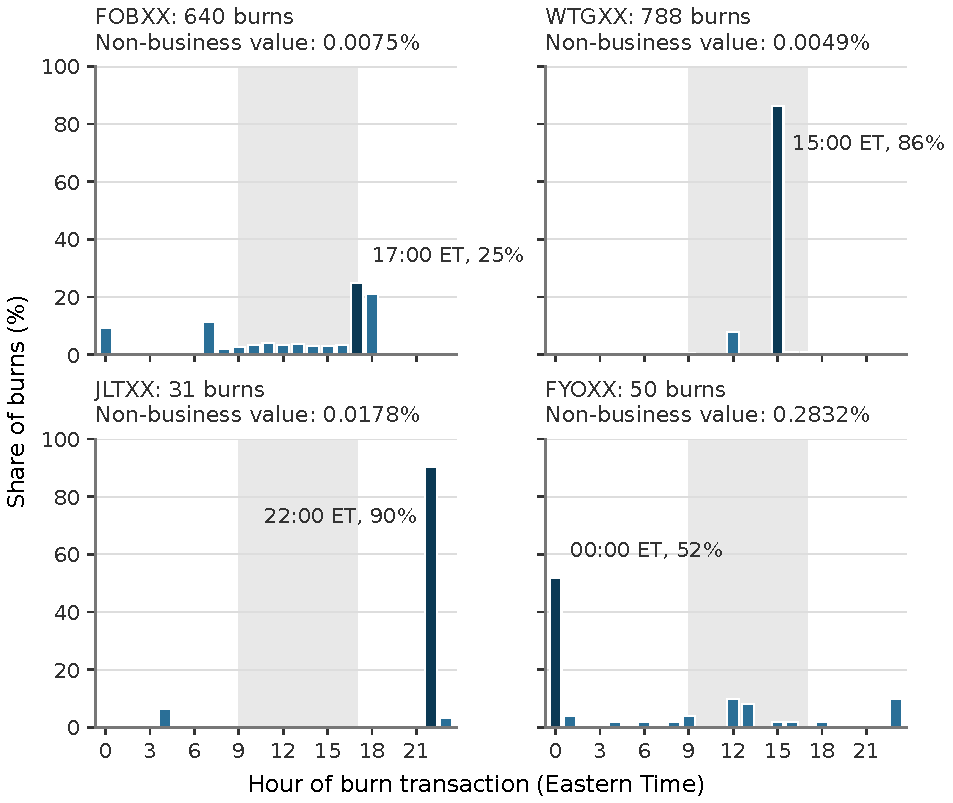
\includegraphics[width=\linewidth]{fig_calendar_revised}
\caption{Share of burn transactions by hour (New York time), 1 January to 30 September 2026, with each fund's non-business share of issuance and redemption value. The darker bar marks the modal hour; the shaded band is 09:00 to 17:00. Event chains only. Source: frozen calendar measures, 16 October 2026; details in Appendix~\ref{app:reproduction}.}\label{fig:calendar}
\end{figure}

Secondary trading is where the token does something new. Of WisdomTree's 68 transfers outside the transfer-agent set, 28 pass through a swap contract that exchanges the token for another in one indivisible, or atomic, transaction, 7 of them on non-business days. Five swaps with Treasury (TSY), a token minted one for one against deposited shares, carry 99.9\% of the route's 200,000 shares; 23 trade small amounts for the USD Coin (USDC) stablecoin at 0.998 to 1.001. Another 22 transfers, not among the 68 because the rules count the custodian contract they use as a transfer-agent wallet, carry about 10 million shares, 13 of them atomically, mostly against USDC or Frax USD at par. Together the two routes carried volume equal to 2.9\% of WisdomTree's filed gross redemptions. Holder-to-holder value came to 9.0\% of gross redemptions, but only 0.028\% without the parent-matched wallet, and to 2.0\% in Franklin, all of it signed with issuer-level keys. Because a transfer can move one owner's tokens without a trade, these gross ratios bound trading from above rather than measure market depth, and redemption through the transfer agent remains the main way out.
% src: data/processed/addl2_summary.csv (swap ALL n_tx 28 atomic 28; TSY 5 tx; USDC 23 tx, price 0.998 to 1.001001; custodian ALL n_tx 22, n_tx_atomic 13; USDC 5 at 1.0; frxUSD 7 at 1.0 to 1.0001); key_numbers.csv addl_swap_n_nonbusiness_day_tr4__WTGXX = 7, addl2_swap_TSY_share_of_route_wtgxx_pct = 99.9406, addl_swap_total_shares__WTGXX = 200124.0, addl2_custodian_wtgxx_amount_all = 10107428.05; addl_contract_venue_ratio.csv venue_share_of_gross_reds_pct = 2.8817; addl_turnover_vs_reds.csv (WTGXX 8.975 / 0.028; FOBXX 1.9836); notes/addl_analysis.md D1 (TSY minted one for one; contract not read)

Atomic execution is not final ownership, and this is where the separation of roles acquires a price. WisdomTree makes a transfer valid at registration and may claw back tokens that do not match its book \citep[pp.~109, 143]{WisdomTreeTMMDF2025}. A buyer who pays USDC for WisdomTree tokens therefore receives the tokens at once but legal title only at registration. The seller bears the stablecoin's par risk, whose historical terms were not examined; the buyer bears registration and clawback risk. On-chain finality is worth less to a buyer when someone other than the holder can still refuse or reverse the entry that counts.
% src: prep_permissions_matrix.csv WTGXX item vii-b (p.109 clawback to align with book-entry records); item i (p.143 valid once registered)

\subsection{Servicing}\label{sec:m4}
Franklin shows one real servicing change: it posts dividend tokens on non-business days. Of 267 classified dividend days in January--September 2026, 78 fall on weekends or holidays, and delivered shares come to about 103\% of estimated accrual, or 28\% if Stellar balances are not seeded. The mint records show where new tokens came from, not who or what triggered them, so automation is not shown. On its 14 non-business dividend days, JPMorgan's dividend mints all occur before 04:00 after a business day, consistent with posting the previous business day's income, weekends and holidays included \citep[p.~28]{JPMorganOnChainLTMMF2026}. WisdomTree's dividend days are all business days, and its delivered shares cover only 32\% of estimated accrual. Monthly reinvestment explains why its dividends cluster \citep[p.~144]{WisdomTreeTMMDF2025}. The shortfall is harder: the prospectus lets holders take cash, and classification may miss some mints, but neither explanation is quantified.
% src: freeze_m4_servicing.csv (FOBXX 267 days, 78 non-business, 103%; JLTXX 86 and 14, 96%; WTGXX 17 days, 31.8574%); freeze_falsifier_verdicts.csv F4 FOBXX stellar_unseeded delivered_pct = 27.6546; addl_divtiming_summary.csv (JLTXX 14 of 14 before 04:00 after a business day)

\subsection{Access}\label{sec:m3}
Low minimums sit beside concentrated holdings, although wallet balances cannot show how many beneficial investors gained access. WisdomTree, with a \textdollar 1 minimum, had 681 holder wallets at 30 September 2026, and Franklin, from \textdollar 20 on Stellar, had 1{,}009. Yet wallets outside the ten largest hold only 0.8\% and 17.6\% of observed holder supply, and because permission, minimum, wallet count and chain move together, no single factor's effect is identified. Franklin's figure could reach 31.1\% if all 108.7 million shares on its unmeasured chains sat outside the top ten.
% src: key_numbers.csv m3_n_nonta_wallets__WTGXX__2026-09-30 = 681, __FOBXX = 1009; m3_nonta_outside_top10_share_pct__WTGXX__2026-09-30 = 0.8029, __FOBXX = 17.6196; f3_uncovered_shares__FOBXX = 108748104.27, f3_worst_case_outside_top10_pct__FOBXX = 31.0908; prep_permissions_matrix.csv item v (minimums)

The filings show the same concentration among record owners. Each filing lists ``each person who owns of record or is known by the fund to own beneficially 5\% or more'' of a class \citep[Item B.10, p.~7]{SECFormNMFP}. In September 2026 one record owner holds 74.5\% of Franklin's token class, 81.5\% of WisdomTree's, 83.6\% of JPMorgan's and 95.1\% of Fidelity's. Only WisdomTree reports a positive beneficial percentage; the other three report zero for every listed owner in every month.\footnote{The specification of the SEC's EDGAR filing system makes both percentages conditionally mandatory and suspends a filing that leaves a decimal empty \citep[PDF pp.~14, 23]{SECNMFP3TechSpec}.} The form defines neither term, so reading the other three funds' dominant owners as nominees or omnibus accounts is an inference; WisdomTree reports its largest record owners as beneficial owners of the same percentages. Pseudonymous wallets cannot supply the investor transparency \citet[p.~3]{Yermack2017} anticipated. Some concentration reflects sponsors' seed capital: WisdomTree's parent-company category held 90.3\% in its first filed month.
% src: freeze_m3_holding.csv 2026-09-30 (FOBXX rec=0.7446; WTGXX rec=0.8147; JLTXX rec=0.8356; FYOXX rec=0.9514); key_numbers.csv addl_ownermatch_top1_minus_dominant_pp__WTGXX = 0.0007, __JLTXX = 0.0018; addl_nmfp_months_with_ben_positive__WTGXX = 28 of 28, __FOBXX/__JLTXX/__FYOXX = 0; data/processed/addl_nmfp_rec_ben.csv WTGXX 2024-06-30 Ultimate Parent Company rec = 0.903

\subsection{Cost}\label{sec:cost}
Fidelity offers the one clean cost comparison: its untokenised Liquidity class (FYHXX) shares OnChain's portfolio and \textdollar 1 million minimum, so their returns differ ``only to the extent that the classes do not have the same expenses'' \citep[Performance]{FidelityTDF2026}.

From January to September 2026, OnChain's seven-day net yield was 2 basis points below Liquidity's on 188 of 189 business days and 1 basis point below on the other. These are business-day reports of overlapping seven-day yields, not 189 independent observations: the period holds about 38 non-overlapping weeks, and the gap is 2 basis points in every one of them. A gap that is constant in every non-overlapping week at the 1-basis-point reporting precision is a persistent price difference, not an estimate with sampling error, so no significance test is reported.
% src: data/processed/exploratory/2026-11-17/fidelity_class_gap_summary.csv paired_mean_gap 2026 = -0.0199 (n 189); paired_gap_value_frequency[-0.02pp] = 188, [-0.01pp] = 1 (2026); weekly_nonoverlapping_sample_n = 38, sd 0.0000 (2026); scripts/24_explore_fidelity_class_gap_2026_11_17.py (exploratory)

Over the full common period from August 2025, the same-date gap averages 9.25 basis points, more than the fee difference, but this is an arithmetic artefact of five reported yields. On OnChain's first five business days, 4 to 8 August 2025, Fidelity filed a seven-day yield of 0.01\% for OnChain against 4.15\% for Liquidity, and those five reports contribute about 7.0 of the 9.25 basis points. Without them the gap is 2.25 basis points, and by October 2025 the gap had settled at about 2 in every month. The launch reports are not lost income. OnChain's shares grew by \textdollar 2{,}691.87 beyond its August subscriptions, consistent with accrual at about 4.09\% from launch; its only holder of record was an affiliated entity; and the first ordinary value is dated 11 August, the first business day seven or more days after launch. The pattern is consistent with an incomplete seven-day calculation window, but the convention is not documented in the held sources.
% src: exploratory/2026-11-17/fidelity_class_gap_summary.csv paired_mean_gap full = -0.0925 (n 294); launch_record_OnChain_net_yield 0.01 on 2025-08-04..08 (Liquidity 4.15); launch_records_contribution_to_full_paired_mean = -0.0704; paired_mean_gap_excl_launch_records = -0.0225 (n 289); monthly_mean_paired_gap 2025-10..2026-09 = -0.0196 to -0.0200; fidelity_class_monthly.csv 2025-08 OnChain (Item B.5 shares 1,002,691.87; Item B.7 subscriptions 1,000,000.00; growth outside flows 2,691.87); raw August 2025 XML Item B.10 OnChain "Affiliated Entity" record 1.0; workflow/reviews/SUPERVISOR17_ECON_AUDIT.md AU-03 (accrual at 4.09% from 4 Aug implies about $2,689; first 4.09% on 2025-08-11; Liquidity launch blank until 2024-12-30); balance_weighted_paired_gap = -0.0208 (full), -0.0200 (2026); fidelity_fee_terms.csv fh OnChain period begins August 4, 2025 (commencement of sale of shares); raw 2026-10-16_FYOXX_N-MFP3_2025-08-31_0001752724-25-213374.xml

The documented expenses account for the 2 basis points. Both classes pay the same gross management fee of 0.25\%; the net difference comes from class-specific waivers and caps. Audited expense ratios net of waivers are 0.18\% for Liquidity in the periods to April 2025 and April 2026 and 0.20\% for OnChain from 4 August 2025 to 30 April 2026 \citep[Financial Highlights]{FidelityTDF2026}. In the 2026 filings, gross yield exceeds each class's net yield by 0.18 and 0.20 percentage points, and filed waivers are about 0.07\% and 0.05\% of average net assets, as in the current fee tables. The contractual caps of 0.18\% and 0.20\% run to 31 August 2027 and are forward-looking terms \citep[Fee Table (Liquidity and OnChain Fund Summaries); Fund Management]{FidelityTDF2026}. Fee terms before June 2026 are not held, and OnChain's higher gross-minus-net spread of 0.24 percentage points in August 2025 is unexplained.
% src: exploratory/2026-11-17/fidelity_fee_terms.csv fh_expenses_net_of_fee_waivers (Liquidity 0.18 FY to 2025-04-30 and 2026-04-30; OnChain 0.20 2025-08-04..2026-04-30); fee_table_* (0.25 management; waivers 0.07 / 0.05; after waiver 0.18 / 0.20); expense_cap_end_date August 31, 2027; fidelity_class_gap_summary.csv gross_minus_net_Liquidity 2026 = 0.1798, gross_minus_net_OnChain 2026 = 0.1997; filed_waiver_annualised 2026 Liquidity 0.0684, OnChain 0.0497 (approximate denominator; quoted to two decimals per SUPERVISOR17_ECON_AUDIT.md AU-02); gross_minus_net_OnChain 2025-08-11..29 = 0.2400 (unexplained; README source gaps)

The prospectus says the difference results from ``separate arrangements for class level services and/or waivers of certain expenses'', and advisory and custodial fees do not vary by class; at present, blockchain transaction fees ``will be borne by the Adviser or its affiliates'' \citep[Fund Management; Use of Blockchain]{FidelityTDF2026}. The 2 basis points are therefore a price for the class, set through class-level service and waiver arrangements, not a measured cost of keeping shares on a blockchain. OnChain holders cannot transfer to each other, so what the class offers is a token record held by the transfer agent, not a secondary trading route; same-day flows between the classes consistent with conversion are listed in Appendix~\ref{app:permissions}. As an illustration, 2~basis points on OnChain's approximate average 2026 balance of \textdollar 128 million come to about \textdollar 19{,}000 over nine months.
% src: exploratory/2026-11-17/fidelity_fee_terms.csv all_inclusive_management_fee_class_difference (Fund Services > Fund Management > Advisory Fee(s)); blockchain_transaction_fees (Fund Basics > Use of Blockchain); converting_shares (Shareholder Information > Converting Shares); fidelity_class_gap_summary.csv same_day_opposite_cross_class_flow 2025-09-02 = 202682868.09|202685559.96; mean_reconstructed_OnChain_balance_on_paired_dates 2026 = 127512956.14 (approx.); ILLUSTRATIVE_income_difference_on_OnChain_balances 2026 = -19164.08; prep_permissions_matrix.csv FYOXX item i (peer-to-peer not permitted)

So the observed gap is 2 basis points, the fee arithmetic accounts for it, class-level service pricing is a plausible mechanism, and no causal cost of tokenisation is identified.

\section{What South African law currently provides}\label{sec:sa}
South African law separates three things a token can blur: securities registration, collective-investment administration and crypto-asset transactions. This section reads the primary texts held at 16 October 2026. The Crypto Asset Manual and the Capital Flow Management (CFM) Regulations are drafts, and the Manual depends on the Regulations being promulgated \citep[p.~2]{SARB2026Circular19}. Scheme deeds, conduct standards, depository rules and anti-money-laundering duties were not examined, and later amendments to the Financial Advisory and Intermediary Services Act (FAIS), the National Payment System Act, and the FMA and CISCA after their 2023 consolidations were not verified. The law is easiest to follow through three ways a tokenised fund unit could reach a South African investor; Table~\ref{tab:sa} summarises the result by function.

\subsection{A domestic fund with its unit register on a ledger}\label{sec:sa_record}
The closest domestic analogue is a money market portfolio under the Collective Investment Schemes Control Act 45 of 2002 (CISCA). Its manager administers issues and cancellations under a deed overseen by a trustee or custodian and may delegate with the registrar's approval \citep[s~1, pp.~1--3; s~4(5)(a), p.~5; s~70(1)(a), p.~26]{CISCA2002}. It must keep proper records, which the registrar may specify by notice \citep[ss~4(4)(b), 114(3)(a), pp.~5, 43]{CISCA2002}. The examined statutes do not expressly bar a ledger-based unit register, though silence is not authorisation and unexamined instruments may constrain its design. The units are already securities: participatory interests and foreign-scheme units fall within the Financial Markets Act 19 of 2012 (FMA) definition \citep[s~1, paras~(a)(v), (b), p.~10]{FMA2012}.

\subsection{A token wrapper over securities in a depository}
\begin{table}[t]
\centering
\small
\caption{South African mechanisms relevant to the observed arrangements}\label{tab:sa}
\begin{tabular}{>{\raggedright\arraybackslash}p{2.7cm}>{\raggedright\arraybackslash}p{6.5cm}>{\raggedright\arraybackslash}p{4.1cm}}
\hline
Function & Mechanism in the examined texts & Consequence \\
\hline
Who records ownership & FMA account entries govern depository transfers; CISCA requires managers' proper records & A wrapper and a manager's unit register need different analysis (Section~\ref{sec:sa_record}) \\
\addlinespace
Who authorises & Statutory register writers are named; draft crypto rules separately cover transactions and routes & Holder signing alone changes no registration authority (Section~\ref{sec:sa_class}) \\
\addlinespace
Payment and calendar & Payment-system finality and deed repurchase cut-offs & Extended processing needs an operating arrangement; designation supplies no central-bank money (Section~\ref{sec:sa_cash}) \\
\addlinespace
Access and holding & Existing foreign-investment controls, issuer eligibility and proposed transaction restrictions & Wallet permission is only one layer of access (Section~\ref{sec:sa_class}) \\
\addlinespace
Servicing & Scheme deed must provide for distributions; offshore treatment depends on the transaction & A dividend token is not automatically a restricted purchase (Section~\ref{sec:sa_class}) \\
\hline
\end{tabular}

\smallskip
\parbox{\linewidth}{\footnotesize\raggedright Primary texts held at 16 October 2026. The Crypto Asset Manual and Capital Flow Management Regulations are proposals. The table distinguishes enacted requirements, proposed restrictions and unexamined scheme instruments; it does not certify a complete implementation.}
\end{table}
For securities in a central securities depository (CSD), the law names both the record and its writer. Transfer is by debit and credit entries in the relevant accounts \citep[s~38(1)(a), p.~48]{FMA2012}, and for a company's uncertificated securities only a participant or CSD may effect it \citep[s~53(1), p.~69]{CompaniesAct2008}. These entries bind third parties and protect a transferee who neither took part in nor knew of a fraud (\citealp[ss~38(3), 41(1), (3), pp.~48--49]{FMA2012}; \citealp[s~53(4), p.~69]{CompaniesAct2008}). Khokha~2, the Reserve Bank's 2022 tokenisation experiment, distinguishes securities constituted as tokens from securities represented by token wrappers \citep[p.~43]{SARB2022Khokha2}. A wrapper over a bond in a licensed CSD could match the bond total exactly, as WisdomTree's tokens match its filings, without transferring the bond: a self-held wallet is not a securities account \citep[s~1, p.~11]{FMA2012}, and clawing back a token does not reverse a statutory entry. What the wrapper holder owns depends on contract, trust or custody arrangements, which may themselves be securities \citep[s~1, para~(e), p.~10]{FMA2012}.

\subsection{A resident holding a foreign fund's token}\label{sec:sa_class}
The Financial Sector Conduct Authority's (FSCA) 2022 declaration makes crypto assets FAIS financial products \citep[cls~1--2, p.~3]{FSCA2022}, and the draft Manual and CFM Regulations use near-identical definitions, the Manual's covering ``distributed ledger or similar technology'', with no securities exclusion (\citealp[A.1, p.~7]{SARB2026CryptoManual}; \citealp[reg~1(1), p.~2]{NT2026CFMDraft}). A token like those examined fits. Within FAIS the overlap is largely harmless, by analogy with FSCA policy on crypto derivatives already regulated as securities (\citealp[p.~4 n.~2; paras~4.10--4.12, p.~10]{FSCA2022Policy}; \citealp[s~1, PDF p.~5]{FAIS2002}); in the exchange-control drafts it has consequences.

Under the draft Manual, transfers between a domestic authorised crypto-asset service provider (CASP) and an offshore CASP, or from a domestic CASP to a non-custodial wallet, are deemed imports or exports where they result in cross-border flows \citep[B.1(A)(ii), p.~24]{SARB2026CryptoManual}; for individuals, any transfer by an authorised CASP to a wallet other than a South African custodial wallet is deemed an export \citep[B.1(C)(iii)(a)(dd), p.~28]{SARB2026CryptoManual}. Resident entities may not enter such transactions \citep[B.1(C)(iii)(b)(dd), p.~31]{SARB2026CryptoManual}, while locally custodied holdings and transfers between authorised CASPs are domestic \citep[B.1(C)(iii)(b)(aa)--(cc), p.~31]{SARB2026CryptoManual}. Individuals' allowance routes run only to a foreign custodial wallet, held with an offshore CASP, or to a non-custodial wallet, whose holder has ``complete control of their private keys and the associated value'' \citep[A.1, p.~8; B.1(C)(iii)(a)(hh), (ii), pp.~28--30]{SARB2026CryptoManual}. On the reading adopted here, those routes may not fit these tokens: issuer revocation and clawback arguably deny complete control, and appointment as a fund's transfer agent is not the home-regulator authorisation that makes an offshore CASP \citep[A.1, p.~9]{SARB2026CryptoManual}. On the counter-reading, a transfer agent is an offshore CASP, bringing its transfers with domestic CASPs within the entity bar. Draft CFM regulation~3 restricts crypto-asset purchases, sales, borrowing and lending above a threshold between persons other than authorised CASPs, subject to permission or exemption \citep[regs~3(1)--(4), 23(6), pp.~6--7, 24]{NT2026CFMDraft}. A subscription could be caught, whereas a dividend token is not automatically a purchase. If draft regulation~12(4)(d), whose grammar is unclear, reaches the acquisition of rights to crypto assets redeemable abroad, a U.S. token would need permission wherever the wallet sits \citep[pp.~15--16]{NT2026CFMDraft}.

The drafts also deem securities transferred abroad when they move ``from a register in the Republic to a register outside the Republic'' (\citealp[reg~1(1), p.~5]{NT2026CFMDraft}; \citealp[A.1, p.~10, in equivalent terms]{SARB2026CryptoManual}). On the interpretation adopted here, the three off-chain registers are abroad from the start, so the rule matters mainly for South African securities placed on a ledger. Franklin's ledger-integrated record has no evident location, although on a counter-reading it sits wherever the transfer agent controls it. Neither draft excludes a token that merely mirrors a domestic register.

In plain terms, if the drafts were adopted as written, a South African resident holding one of these tokens would hold a crypto asset as well as a foreign fund share. A company could not move it across the border through a crypto provider; an individual could, through an authorised provider within the annual allowances, if those routes fit these wallets. Direct dealings with the fund could also need permission, on the readings of regulations~3 and~12(4)(d) given above.

Existing controls apply alongside. The 1961 Exchange Control Regulations require Treasury permission for specified non-resident register changes and for dealing in controlled securities \citep[reg~14(1)--(3), pp.~16--17]{ExConRegs1961}, although their application to a self-held token was not examined, and conventional routes include a corporate portfolio allowance and institutional investors' foreign-exposure limit \citep[B.2(C)(iii), pp.~60--61; B.2(H)(iv), p.~73]{ADManual2026}. Fund terms also matter: JPMorgan's fund ``is not intended for foreign shareholders'' \citep[p.~30, a tax warning]{JPMorganOnChainLTMMF2026}, and WisdomTree generally sells only to U.S. residents \citep[Your Account]{WisdomTreeTMMDF2025}.

Overlap is not automatically conflict. FMA section~3 gives qualified priority for actual inconsistencies \citep[ss~3(3)--(5), p.~15]{FMA2012}, but it does not exclude securities from the crypto definitions, and whether it reaches subordinate exchange-control instruments was not examined. Rwanda, by contrast, brings real-world-asset tokens within its virtual-asset definition but expressly excludes capital-market securities \citep[arts~4(2)(a), 4(3)(c), pp.~20--21]{Rwanda2026VirtualAssets}.

\subsection{The cash leg}\label{sec:sa_cash}
The National Payment System Act gives finality to settlement through the Reserve Bank or designated systems \citep[ss~1, 4A(1), 5, pp.~3, 6, 8]{NPSAct1998}, but designation does not itself create central-bank money, and the draft CFM Regulations exclude crypto assets, and so on their wording a privately issued stablecoin, from ``currency'' \citep[reg~1(1), p.~2]{NT2026CFMDraft}. CISCA deeds fix repurchase cut-offs and distributions \citep[Sched.~1 items~1(f), 2(b)--(c), p.~45]{CISCA2002}. None of these supplies a rand settlement asset on a token ledger.
% src: held FMA consolidation ss1,3,6,36--41; CISCA ss1,4,22,65,70,97,114/Schedule1; Manual A1/B1; draft CFM regs1,3,12,23; table rows below summarise these subsections


\section{Which route should South Africa take?}\label{sec:policy}
What follows is my recommendation, not a statement of current law or a permission to launch any product. The three routes need not be exclusive; IOSCO records members combining new laws with sandboxes \citep[p.~63]{IOSCO2025}.

A security-token definition would close the gap Khokha~2 identified: security tokens ``are not currently defined in the FMA, which makes their regulatory treatment uncertain'' \citep[p.~43]{SARB2022Khokha2}. For tokenised fund units, though, classification is largely not the problem, because they are already participatory interests and FMA securities. A definition would not say how title passes, since FMA transfer effects attach to register entries, nor supply a cash leg, and an FMA carve-out would not automatically bind exchange-control instruments. Franklin shows a further risk: legislating title for a ledger does not give holders control if issuer-level keys sign.

A technology-neutral reading is probably the cheapest and quickest route and the one most IOSCO members take \citep[p.~62]{IOSCO2025}; Khokha~2 likewise asks for legislation that is ``technology neutral and principle based'' \citep[p.~44]{SARB2022Khokha2}. A CISCA manager could keep a ledger as, or alongside, its proper records, and the register-governs model of WisdomTree, JPMorgan and Fidelity fits without new law. It leaves the drafts' technology-based crypto definitions untouched, however.

A pilot can produce the evidence the four funds cannot, and existing powers would support one. The registrar may exempt managers in the public interest, exempt categories of schemes from deed requirements and specify records \citep[ss~22, 97(2), 114(3)(a), pp.~11, 35, 43]{CISCA2002}. The FSCA must consider ``the desirability of facilitating innovation'' and may impose conditions, issue guidance and grant time-limited exemptions \citep[s~6(3)(b)(iii), (h), (k), (m), pp.~17--18]{FMA2012}. On exchange control, Treasury permission is available under the 1961 Regulations \citep[reg~14(1), p.~16]{ExConRegs1961}, and draft CFM regulation~23 would add class exemptions and permissions \citep[reg~23(1)--(2), p.~23]{NT2026CFMDraft}. On my reading, these powers remove duties rather than create rights: an exemption probably cannot give a token entry the third-party effect that FMA sections~38(3) and~41 give a depository entry, and FMA exemptions require financial or other hardship or prejudice and must not conflict with the public interest.

I therefore recommend three steps. First, apply existing law technology-neutrally now: a tokenised unit is a participatory interest, and the record named in the scheme deed and kept by the manager should be treated as the governing register. Second, run a conditional pilot under existing powers. It should test daily reconciliation of token supply to the register, signer and key records against the register-writer, correction and clawback governance, rand settlement timing, beneficial-investor reach rather than wallet counts, and costs against a matched untokenised class, as Fidelity's design allows. Safeguards should include a governing record named in the deed, published token addresses, disclosed issuer powers and key arrangements, caps on volume and participants, and wallets hosted by an authorised CASP (South African custodial wallets) so that transfers stay domestic. Sustained reconciliation without breaks, measured savings against the control class, no investor-rights incidents and a demonstrated need for statutory title effect would justify wider adoption or legal change. Third, clarify the draft exchange-control instruments, which the Reserve Bank described in July 2026 as under review \citep[p.~2]{SARB2026Circular19}. Under the securities statutes these units are already classified; the drafts add a second classification as crypto assets, which a narrow clarification can remove, while title and the register remain matters for the pilot. As Khokha~2 anticipated, how a crypto framework would ``interact with the securities regulatory framework'' needs settling \citep[p.~43]{SARB2022Khokha2}: treat tokenised FMA securities and CISCA participatory interests under the securities provisions, or add a priority rule, and give a register-location rule that works for ledgers.

The strongest objection is that a carve-out invites relabelling, and that drafters may want to catch every transfer to a non-custodial wallet whatever the instrument. That risk is better met by tying the carve-out to instruments already regulated as securities than by leaving a fund unit in two regimes at once.

\section{What the evidence cannot show}\label{sec:limits}
The evidence describes four young funds without a counterfactual. It does not measure what tokenisation saves in settlement or servicing, whether it deepens liquidity, or whether it brings in more beneficial investors. The Fidelity comparison prices a class rather than isolating a technology.

Matching totals cannot show which record was written first, and none of the data identifies a common producing system. Mint records reveal the source of new tokens but not who or what triggered them, so neither automated servicing nor earlier spendable cash is shown. Token-event dates are not cash-settlement times. Signatures identify the keys that authorised a transfer; who held those keys or gave the instruction remains unknown, and validators are outside the analysis. The signature and contract-code analysis is exploratory.

Coverage is uneven. Fidelity has not confirmed its token address, Franklin's Aptos chain and early Stellar history are missing, and JPMorgan's history is short. The original thresholds were recorded after the calibration window, and several verdicts depend on choices made with that window in view (Appendix~\ref{app:verdicts}). Record authority comes from prospectus terms rather than a separate analysis of U.S. property law.

The South African analysis covers primary texts held at 16 October 2026. Two of them are drafts, and scheme deeds, conduct standards and depository rules were not examined. The policy recommendation is a judgment on that evidence; no welfare effect has been demonstrated.

\section{Conclusion}\label{sec:conclusion}
The token ledger has not simply taken over the transfer agent's work, nor merely copied it. It has moved particular roles in particular funds. At Franklin the blockchain is part of the legal ownership record, but issuer-level keys sign holders' transfers. At WisdomTree holders sign, but ownership changes only when the transfer agent registers the transfer. Being a party to a transfer, authorising it and making the legally effective entry are different things, and the funds show that they come apart in both directions.

That separation is also the economic story. Primary processing still runs on bank days. The new secondary routes are mostly atomic but small, and their finality is limited by registration and clawback. Franklin's weekend dividend posting is a genuine servicing change, while low minimums sit beside highly concentrated ownership. Fidelity's two-basis-point class difference is matched by documented waivers and caps; it prices the class and says little about what the blockchain itself costs.

For South Africa, the funds point to the record and its writer rather than to classification. I recommend reading existing law technology-neutrally now, running a conditional pilot under existing powers to gather the evidence these funds cannot supply, and narrowly clarifying the draft exchange-control instruments so that tokenised securities and fund units are not caught twice. A broad security-token definition would answer a question the funds suggest is not binding.

\clearpage
\phantomsection
\addcontentsline{toc}{section}{References}
{\interlinepenalty=10000
\bibliography{drafts/independent/references_revised}}

\newpage
\appendix

\section{Glossary and code key}\label{app:glossary}
\paragraph{Terms.} \emph{Transfer agent}: the firm that keeps a fund's register of shareholders. \emph{Transfer-agent set}: the wallets inferred to belong to the transfer agent, because they create or destroy tokens, briefly hold redemptions before burning them, or pass on new issuance (Appendix~\ref{app:rules}). \emph{Mint} and \emph{burn}: creating and destroying tokens. \emph{Atomic exchange}: two token movements that settle in one transaction or not at all. \emph{Safe wallet}: a contract that holds tokens and moves them on its owners' signatures. \emph{Stellar signer weight}: each key on a Stellar account carries a weight; an account whose own (``master'') key has zero weight can be operated only by its other signers. \emph{Calibration window}: the July--September 2026 data used to set the rules and thresholds (called the pilot in earlier project records). \emph{Form \mbox{N-MFP3}}: the monthly SEC report of a money market fund's holdings, flows, yields and large owners.

\paragraph{Codes used in the appendices and project records.}
\begin{center}
\footnotesize
\begin{tabular}{>{\raggedright\arraybackslash}p{2.2cm}>{\raggedright\arraybackslash}p{11.6cm}}
\hline
Code & Plain name \\
\hline
TA & Transfer agent \\
TR-1--TR-4 & Timing rules: New York dating and month-end cutoff; parked redemptions; next-day dividend mints; non-business days \\
TR-5 & Wallet-role rule (transfer-agent set, contracts, holders) \\
TR-6 & Dividend-classification rule \\
M0, F0 & Reconciliation measure and its test (token supply against filed shares) \\
M1, F1 & Transfer-party measure and its benchmark \\
M2, F2 & Processing-calendar measure and its test \\
M3, F3 & Holdings-concentration measure and its benchmark \\
M4, F4 & Dividend-servicing measure and its test \\
M5 & Permission-against-use comparison (descriptive) \\
F-SA & South African legal test \\
K1--K5 & Functions: record authority; operational control; payment and calendar; access and holding; servicing \\
FOBXX & Franklin OnChain U.S. Government Money Fund \\
WTGXX & WisdomTree Treasury Money Market Digital Fund \\
JLTXX & JPMorgan OnChain Liquidity-Token Money Market Fund \\
FYOXX, FYHXX & Fidelity Treasury Digital Fund, OnChain and Liquidity classes \\
\texttt{0x0c561ed8} & The WisdomTree wallet matched to the parent company \\
\hline
\end{tabular}
\end{center}

\section{Original tests, verdicts, power and sensitivities}\label{app:verdicts}
\paragraph{The original hypothesis and its tests.} The original follower hypothesis predicts that only the transfer agent writes, that the chain follows the register, that processing keeps the business calendar and that holding stays mostly intermediated, with distribution servicing as an exception. These predictions require different evidence: F0 tests aggregate consistency rather than chronology, M1 classifies parties, and no falsifier directly tests intermediated holding. Table~\ref{tab:measures} preserves the six original measures and thresholds, recorded before the raw freeze. % src: git commit 76e76d2 (2026-10-16 17:24 +0200; adds notes/preregistration.md); raw freeze commit 07afeb3 (2026-10-16 22:42 +0200)
M1 counts non-dividend transfers with neither party in the transfer-agent set, and its pre-specified sensitivity counts all non-dividend events. Who signed is read separately, and neither shows who instructed a transfer. M1's thresholds provide a descriptive benchmark; they do not measure liquidity or the transfer agent's validation and registration functions. % src: Aquilina2025BIS115 printed p.2 (PDF p.4); thresholds from notes/preregistration.md F1 row
F-SA is decided from South African primary texts and is not triggered: neither draft excludes a mirroring token from the crypto-asset definition, and the register-location rule concerns securities transfers, not the token's classification (Section~\ref{sec:sa}). The transfer, calendar and dividend measures are pooled over 1 January to 30 September 2026, the window common to all chains.

\begin{table}[htbp]
\centering
\small
\caption{Measures and pre-specified falsifiers}\label{tab:measures}
\begin{tabular}{>{\raggedright\arraybackslash}p{0.9cm}>{\raggedright\arraybackslash}p{5.9cm}>{\raggedright\arraybackslash}p{7.2cm}}
\hline
 & Measure (unit) & The claim is refuted for a fund if \\
\hline
M0 & Consistency test: on-chain supply on all chains against \mbox{N-MFP3} class shares, after TR-1 to TR-3 (fund-month) & F0: more than two out-of-sample months show a gap above 0.10\% of class shares; a month missing a chain counts only if covered supply already exceeds \mbox{N-MFP3} by more than 0.10\% \\
M1 & Party measure: share of non-dividend transfer value and count with neither side in the TA set; the upper bound adds unlabelled contracts (event) & F1: the upper bound is at least 5\% of value or at least 10\% of count \\
M2 & Share of issuance and redemption value on non-business days; modal burn hour; same-day match to \mbox{N-MFP3} subscriptions (event, fund-day) & F2: at least 10\% of value falls on non-business days \\
M3 & Supply in TA wallets; \mbox{N-MFP3} record-owner categories; for FOBXX and WTGXX, the share of non-TA supply outside the ten largest wallets (quarter-end) & F3: wallets outside the top ten hold at least 25\% at 30 September 2026 \\
M4 & Dividends delivered as on-chain mints: share of estimated accrual, dividend days including non-business days, lag (event) & F4: dividend mints occur only on business days, in TA batches, with a median lag of at least one business day \\
M5 & Prospectus permission against measured use (fund by function) & Descriptive; no falsifier \\
F-SA & South African primary texts held at 16 October 2026 (legal) & F-SA: a primary text excludes a token that only mirrors a South African register from the crypto-asset definition, or the register-location test treats such a token as domestic \\ % src: notes/preregistration.md F-SA row
\hline
\end{tabular}

\smallskip
\parbox{\linewidth}{\footnotesize\raggedright Notes: TA denotes the transfer agent. F0 measures aggregate consistency, F1 transfer-party roles and F3 wallet concentration; none directly identifies chronology, authorisation or participation effects. F4 uses the three conditions jointly. Thresholds followed the calibration window but preceded the raw freeze; Appendix~\ref{app:reproduction} records the chronology.} % src: notes/preregistration.md §4.5 "Claim at risk" column (F0 to F4, F-SA); git log 76e76d2 2026-10-16 17:24:30 +0200; git log 07afeb3 2026-10-16 22:42:27 +0200
% src: notes/preregistration.md §4.4 and §4.5 (thresholds); notes/preregistration_implementation_notes.md Fix 6 (one-sided rule), IMPL-15, IMPL-21
\end{table}

\paragraph{Calibration, deviations and power.}\label{app:calib} A feasibility study on July to September 2026 data (the calibration window) informed the timing rules and thresholds. F0 is therefore tested only on earlier \mbox{N-MFP3} months. Because the calibration months fall inside the window of F1 to F4, those tests were re-run on January to June 2026, and every verdict that can still be tested is unchanged, even with wallet roles reassigned on events to 2 July (Table~\ref{tab:verdicts}). % src: data/processed/addl_oos_verdicts.csv; key_numbers.csv addl_oos_matches_full__*__main and __horizon (all yes; FYOXX F4 no, NOT TESTABLE); addl_oos_role_changes_horizon_vs_frozen = 1
Eleven implementation choices were made with the calibration data in view (Appendix~\ref{app:rules}), and four historical coded verdicts depend on one of them (Table~\ref{tab:verdicts}). % src: data/processed/freeze_falsifier_verdicts.csv (robustness rows); key_numbers.csv f0_robust__WTGXX, f1_robust__FOBXX, f4_robust__WTGXX, f4_robust__FYOXX
Exploratory analyses on logged additions to the vintage changed no frozen measure, rule or verdict. % src: data/raw/ADDITION_MANIFEST_2026-10-17.csv; data/raw/ADDITION_MANIFEST_2026-10-18.csv and data/README.md ADDITION 2; notes/addl_analysis.md header ("No frozen file, measure, rule or verdict was changed")
F4 requires three conditions jointly: business-day-only mints, TA batches and a median lag of at least one business day. Where lag is unavailable, the historical code scores only the calendar and batch components. Franklin and JPMorgan fail the calendar condition, so the full refuting conjunction is not met despite unknown lag. WisdomTree meets the calendar and batch conditions, leaving full refutation unresolved because lag is unknown; even its historical partial result reverses under a one- or three-hour batch span. Fidelity's coded refutation is uninformative after failed reconciliation. Similarly, F2 records token-event dates without cash-settlement timestamps. % src: notes/preregistration.md §4.5 F4 (three conditions); prep_permissions_matrix.csv item iii (bank channels, all four)

\paragraph{Earlier-month checks.} Fidelity's F4 becomes untestable in January--June without month-start dividend mints; Franklin's missing-chain concentration upper bound exceeds F3's threshold at both dates, at 32.4\% in June and 31.1\% in September. % src: key_numbers.csv addl_oos_worst_case_outside_top10_pct__FOBXX__F3__main = 32.3674 (2026-06-30); f3_worst_case_outside_top10_pct__FOBXX = 31.0908; addl_oos_n_dividend_days__FYOXX__F4__main = 0

\paragraph{Date-order checks.} \mbox{N-MFP3} records flows ``as of the trade date'' without timestamps \citep[p.~6]{SECFormNMFP}. No selected matched WisdomTree or Fidelity mint or burn precedes its filed date, although within-day order is unknown. Fidelity's selected mints follow on 6 of 28 subscription days and burns on 36 of 44 redemption days, whereas JPMorgan mints precede on 4 of 97 days and Franklin's previous-day burns match on 54 of 173 redemption days. Franklin's issuance matches same-day \mbox{N-MFP3} subscriptions on 0 of 187 business days. These comparisons cannot establish which ownership record was written first. % src: data/processed/addl_ordering_summary.csv; key_numbers.csv m2_flowmatch_days_same_day_match__FOBXX = 0, m2_flowmatch_nmfp_business_days__FOBXX = 187, diag_m2_flowmatch_div_added_match_days__FOBXX = 2. Selected date matching is exploratory, not observed registration chronology.

\paragraph{WisdomTree party-measure sensitivities.} Table~\ref{tab:wtgxxsens} completes Table~\ref{tab:wtgxx}. Every rule variant preserves the WisdomTree refutation, but the pre-specified all-events denominator reverses it. Counting the debited wallet as a burn's origin puts the parent-matched wallet, which the transfer agent's burns debit, in the TA set, and gives the same bounds as removing it from the numerator.

\begin{table}[htbp]
\centering
\footnotesize
\caption{WisdomTree party-measure sensitivities}\label{tab:wtgxxsens}
\begin{tabular}{>{\raggedright\arraybackslash}p{8.4cm}>{\raggedright\arraybackslash}p{2.6cm}>{\raggedright\arraybackslash}p{3.4cm}}
\hline
 & All wallets & Without \texttt{0x0c561ed8} \\
\hline
Upper bound, lowest and highest rule variant: value & 11.2\% to 77.8\% & Not reported \\ % src: freeze_falsifier_verdicts.csv F1 WTGXX burn_origin_transfer_from upper_value_pct = 11.2275, hop_leg_off upper_value_pct = 77.7847 (all variants FAIL)
Upper bound counted against all events, issuance and redemption included (pre-specified sensitivity): value; count & 3.4\%; 2.1\% & Not reported \\ % src: key_numbers.csv m1_upper_share_value_pct__WTGXX__pooled__all_events = 3.4462, m1_upper_share_count_pct__WTGXX__pooled__all_events = 2.1092
Upper bound, 1 January to 30 June 2026 (out of sample): value; count & 39.1\%; 41.3\% & Not reported \\ % src: key_numbers.csv addl_oos_upper_share_value_pct__WTGXX__F1__main = 39.1361, addl_oos_upper_share_count_pct__WTGXX__F1__main = 41.3462
Upper bound, transfers of 100 shares or more: value; count & Not reported & 11.2\%; 26.5\% \\ % src: key_numbers.csv addl_f1minsize_upper_share_value_pct__WTGXX__min_100_shares__excl_wallet_numerator = 11.2275, addl_f1minsize_upper_share_count_pct__WTGXX__min_100_shares__excl_wallet_numerator = 26.4706
\hline
\end{tabular}

\smallskip
\parbox{\linewidth}{\footnotesize\raggedright The first two rows are frozen measures; the others are exploratory.} % src: freeze_falsifier_verdicts.csv F1 WTGXX burn_origin_transfer_from (upper 11.2275, 37.4269; lower 0.0864, 18.1287); data/processed/addl_pm_wallet_profile.csv (burns from 0x0c561ed8 sent by TA wallet 0x726d3b3e via burn(address,uint256))
\end{table}

\paragraph{Coded verdicts.} Table~\ref{tab:verdicts} distinguishes the coded results from what the measures identify. ``Claim survives'' means its stated falsifier was not met, not that the claim is proved. F4's historical partial labels omit unavailable lag.

{\footnotesize
\setlength{\parskip}{0pt}
\begin{longtable}{>{\raggedright\arraybackslash}p{1.1cm}>{\raggedright\arraybackslash}p{1.4cm}>{\raggedright\arraybackslash}p{2.5cm}>{\raggedright\arraybackslash}p{2.8cm}>{\raggedright\arraybackslash}p{2.9cm}>{\raggedright\arraybackslash}p{2.1cm}}
\caption{Original falsifier results, test power and reversing sensitivities}\label{tab:verdicts}\\
\hline
Test (K) & Fund & Verdict on the claim & Power & Reversed by & Post-calibration choice \\
\hline
\endfirsthead
\multicolumn{6}{l}{\textit{Table~\thetable\ (continued)}}\\[3pt]
\hline
Test (K) & Fund & Verdict on the claim & Power & Reversed by & Post-calibration choice \\
\hline
\endhead
\multicolumn{6}{p{14.8cm}}{\textit{F0, consistency (K1). Original claim: the chain copies the register in aggregate. Refuted if more than two test months miss by over 0.10\%.}} \\*
F0 (K1) & FOBXX & Not testable & None: 0 of 25 months complete (Aptos missing in each) & None & No \\ % src: key_numbers.csv coverage_oos_months_incomplete__FOBXX = 25, coverage_oos_missing_chain_sets__FOBXX (Aptos in every month), f0_n_complete__FOBXX = 0
F0 (K1) & WTGXX & Claim survives (0 of 10 months) & 10 complete months of 25 & Counting every next-day dividend mint (refuted, 6 of 10) & Yes: which dividend mints count \\
F0 (K1) & JLTXX & Not testable & None: 2 months (both 0.0000\%) & None & No \\ % src: notes/freeze_results.md §2b JLTXX; key_numbers.csv f0_n_oos_months__JLTXX = 2
F0 (K1) & FYOXX & Claim refuted (11 of 11 months) & 11 complete months; address unconfirmed & None & No \\
\hline
\multicolumn{6}{p{14.8cm}}{\textit{F1, transfer parties (K2). Original claim: only the TA writes; this measure counts parties. Refuted if others' transfers reach 5\% of value or 10\% of count.}} \\*
F1 (K2) & FOBXX & Threshold exceeded by party; issuer-level signers & Stellar only; other chains precluded; issuer-level keys sign all 44 observed transfers outside the TA set (Section~\ref{sec:writes}) & Counting issuance and redemption; Stellar redeemers put in the TA set & Yes: role of Stellar redeemers \\ % src: freeze_falsifier_verdicts.csv F1 FOBXX stellar_burner_leg_on upper_value_pct = 0.0009, upper_count_pct = 8.6957 PASS-for-claim; key_numbers.csv f1_robust__FOBXX
F1 (K2) & WTGXX & Claim refuted & Four chains with events; value rests on one wallet and on contracts (Table~\ref{tab:wtgxx}) & Counting issuance and redemption (pre-specified) & No \\
F1 (K2) & JLTXX & Not testable & Not applied: four holders under the pre-specified restriction; 8 of 39 transfers outside the TA set & None & No \\ % src: key_numbers.csv m1_upper_share_count_pct__JLTXX__pooled__transfers_only = 20.5128, m1_n_events__JLTXX__pooled__transfers_only = 39, m3_n_nonta_wallets__JLTXX__2026-09-30 = 4
F1 (K2) & FYOXX & Claim survives (divergent record) & Weak: few wallets; peer-to-peer not permitted & None & No \\
\hline
\multicolumn{6}{p{14.8cm}}{\textit{F2, calendar (K3). Claim: issuance and redemption keep the business calendar. Refuted if 10\% of value falls on other days.}} \\*
F2 (K3) & FOBXX & Claim survives & Chains with event histories; none on Aptos, Avalanche, Base; issuance never matches the same-day \mbox{N-MFP3} subscription & None & No \\ % src: key_numbers.csv m2_flowmatch_days_same_day_match__FOBXX = 0, m2_flowmatch_nmfp_business_days__FOBXX = 187; notes/freeze_results.md section 4 FOBXX diagnostic
F2 (K3) & WTGXX & Claim survives & Chains with event histories; none on Avalanche, Base, Optimism, Plume & None & No \\
F2 (K3) & JLTXX & Claim survives & Full (Ethereum; Solana added 1 October 2026, after the window) & None & No \\ % src: notes/token_contracts.md JLTXX (497 supplement 1 Oct 2026 adds Solana)
F2 (K3) & FYOXX & Claim survives (divergent record) & Full (Ethereum only) & None & No \\
\hline
\multicolumn{6}{p{14.8cm}}{\textit{F3, concentration benchmark (K4). Original claim: low minimums bring no breadth. Refuted if wallets outside the ten largest hold at least 25\%.}} \\*
F3 (K4) & FOBXX & Claim survives (worst case unsettled) & Covered chains only & All shares on unmeasured chains outside the top ten & No \\
F3 (K4) & WTGXX & Claim survives & Covered chains & None & No \\ % src: key_numbers.csv f3_worst_case_outside_top10_pct__WTGXX = 0.8998
F3 (K4) & JLTXX & Not tested & Defined for low-minimum funds & Not applicable & Not applicable \\
F3 (K4) & FYOXX & Not tested & Defined for low-minimum funds & Not applicable & Not applicable \\
\hline
\multicolumn{6}{p{14.8cm}}{\textit{F4, servicing (K5). Original claim: servicing is automated on chain, the hypothesis's exception. Refuted if dividend mints fall only on business days, in TA batches, at least a business day late.}} \\*
F4 (K5) & FOBXX & Historical partial survival; full conjunction not met (calendar) & Lag not identified & None & No \\
F4 (K5) & WTGXX & Refuted as historically coded (partial); full conjunction unresolved & Lag not identified & Widening a TA batch to a one- or three-hour span & Yes: TA batch definition \\
F4 (K5) & JLTXX & Historical partial survival; full conjunction not met (calendar) & Lag not identified & Mint-date convention (exploratory) & No \\ % src: data/processed/addl_divtiming_summary.csv JLTXX 14 of 14 non-business days early after a business day
F4 (K5) & FYOXX & Refuted as coded, but uninformative & Divergent record & Dropping the month-start dividend rule (not testable) & Yes: month-start dividend rule \\
\hline
\multicolumn{6}{p{14.8cm}}{\footnotesize\raggedright Notes: coded outcomes refer to the original benchmarks, not demonstrated economic effects. F4 partial coding omits unavailable lag; the full conjunction is interpreted under ``Calibration, deviations and power'' above. K codes are listed in Appendix~\ref{app:glossary}.}\\
\end{longtable} % src: data/raw/ADDITION_MANIFEST_2026-10-17.csv; data/raw/ADDITION_MANIFEST_2026-10-18.csv; data/README.md ADDITION CP42, cycle 2 D9, cycle 4 (scripts/19_addl_swap_and_owner.py), ADDITION 2 (scripts/22_addl2_cashlegs.py); notes/addl_analysis.md header, A1, A4, A6, A7, C1 to C6, D1
% src: data/processed/addl_oos_verdicts.csv; key_numbers.csv addl_oos_upper_share_value_pct__WTGXX__F1__main = 39.1361, addl_oos_upper_share_count_pct__WTGXX__F1__main = 41.3462, addl_oos_worst_case_outside_top10_pct__FOBXX__F3__main = 32.3674 (snapshot 2026-06-30), f3_worst_case_outside_top10_pct__FOBXX = 31.0908 (2026-09-30), addl_oos_n_dividend_days__FYOXX__F4__main = 0
% src: data/processed/freeze_falsifier_verdicts.csv (main, sensitivity, per-chain, bound and robustness rows); key_numbers.csv f0_*, f2_verdict__*, f0_robust__*, f2_robust__*, f1_robust__*, f3_robust__*, f4_robust__*; notes/claim_home.md Correction (2026-10-17); freeze_m2_calendar.csv chains_without_events
}

\section{Classification rules and calibration choices}\label{app:rules}

\paragraph{TR-1 to TR-4, timing.} Events are dated in \mbox{America/New\_York} time (ET), and a month ends at 23:59:59 ET on the \mbox{N-MFP3} report date (TR-1); a cutoff at 23:59:59 in Coordinated Universal Time is a sensitivity. In the two funds whose burn wallet holds no lasting balance, JPMorgan's and Fidelity's, a balance parked in a TA burn wallet and burned by the end of the next ET business day counts as redeemed on the day it arrived (TR-2). Dividend shares that \mbox{N-MFP3} records on business day $d$, the report date, and that the chain mints by the end of the next ET business day count as on chain at $d$ (TR-3). In the main specification TR-3 adds only TR-6 rule (iii) dividends, the only mints matched to an \mbox{N-MFP3} subscription, and it cannot be applied on chains without an event history. Non-business days are Saturdays, Sundays and Fedwire holidays from 2024 to 2026 (TR-4).
% src: notes/preregistration.md §4.4 TR-1 to TR-4; notes/preregistration_implementation_notes.md IMPL-2, IMPL-3, IMPL-4 (d+1 = next ET business day), IMPL-4b (TR-3 scope; chains without event history), IMPL-11; TR-1 UTC sensitivity (implementation notes, sensitivity table "clock=UTC")

\paragraph{TR-5, wallet roles.} Roles are assigned separately on each chain, with the legs applied in order. The TA set contains: (a) the mint source, which is the zero address on EVM chains and Solana and the issuer account on Stellar; (b) module contracts listed by the issuer, which only Franklin publishes; (c) any account that sends a burn transaction on an EVM chain; (d) any address that burns more than half of its non-mint inflow value within two ET business days of arrival (parking); and (e) any address that receives an issuance mint and forwards at least 95\% of it on the same ET day to wallets other than burn or parking wallets (distribution hop). The legs can sweep in a third-party contract, as the distribution-hop leg does with one custodian contract (\texttt{FrxUSDCustodian\allowbreak WithReceiver}) in WisdomTree; moving it out leaves WisdomTree's verdict unchanged (Table~\ref{tab:wtgxx}). A contract is an address with code that is outside the TA set, or a Soroban contract address on Stellar. Every other address is a holder. The rule is deterministic, unlike the role classifier of \citet[p.~5]{Luo2025}, which learns from noisy name-based labels. Solana program accounts cannot be told apart from wallets, so they count as holders unless a TA leg applies. M1 takes holder-to-holder flows as its lower bound, adds holder-to-contract flows for the main value, and adds contract-to-contract flows for the upper bound. F4's TA-batch condition is met by dividend mints from leg (a)'s mint source (Table~\ref{tab:calibchoices}, row 10), so it shows the source of a mint and leaves open who triggered it.
% src: notes/preregistration.md §4.4 TR-5; notes/preregistration_implementation_notes.md IMPL-1, IMPL-5, IMPL-6, IMPL-7, IMPL-7b, IMPL-15, IMPL-16, IMPL-19, Fix 1; key_numbers.csv addl_reclass_m1_upper_share_value_pct__WTGXX__reclass__with_wallet = 47.5195; data/processed/addl_frax_custodian.csv

\paragraph{TR-6, dividend mints.} A mint is a dividend under any of three rules. (i) It belongs to a same-ET-day batch paid to two or more existing holders whose amounts correlate with prior balances at $\rho \geq 0.95$, and it is no larger than five times prior balance $\times$ (seven-day net yield$/365$) $\times$ days since that address's last mint. (ii) Any other mint lies within 2\% of that accrual. (iii) In a single-chain fund, the day's unlabelled mints equal the \mbox{N-MFP3} gross subscription for that date to within 0.01 shares, on the first ET business day of a month. All other mints are issuance. On Stellar, prior balances are seeded at 1 January 2026 by backing out from current balances, and TR-5 and TR-6 use Stellar events from that date. Events between 1 September and 31 December 2025 enter only month-end supply.
% src: notes/preregistration.md §4.4 TR-6; notes/preregistration_implementation_notes.md IMPL-1b, IMPL-8, IMPL-8c (Fix 2, k = 5), IMPL-9, IMPL-10, Fix 3; data/README.md FREEZE VINTAGE (Stellar)

\paragraph{Choices made with the calibration window in view.} Table~\ref{tab:calibchoices} lists the eleven choices. For choices 1--10 the reported sensitivities vary the stated implementation against the main specification on the frozen data. Choice 11 instead records the one-sided rule for incomplete months; no parameter sensitivity is reported for it.

\begin{table}[htbp]
\centering
\small
\caption{Implementation choices made after the July to September 2026 calibration window}\label{tab:calibchoices}
\begin{tabular}{>{\raggedright\arraybackslash}p{0.4cm}>{\raggedright\arraybackslash}p{3.6cm}>{\raggedright\arraybackslash}p{5.4cm}>{\raggedright\arraybackslash}p{4.6cm}}
\hline
 & Rule & Main specification & Sensitivity reported \\
\hline
1 & TR-6 Stellar balances & Seeded at 1 January 2026 & Unseeded \\
2 & TR-3 scope & Only rule (iii) dividends added & All next-day dividend mints added \\
3 & TR-5 burn origin & EVM transaction sender; leg off on Stellar and Solana & Debited wallet on EVM; Stellar leg on \\
4 & TR-5 hop & Forwards to burn or parking wallets excluded & Included \\
5 & TR-6 (i) outlier guard & Dropped & Guard at three times the batch median \\
6 & TR-6 (i) accrual cap & Five times one period's accrual & Three, ten, no cap, day-aware cap \\
7 & TR-6 (iii) & First business day of a month; 0.01 shares & Rule off; 1 and 100 shares; monthly accrual size test \\
8 & TR-5 hop trigger & Issuance mints only & All mints; hop leg off \\
9 & M4 lag & Only where \mbox{N-MFP3} dates the accrual (FYOXX), counted from the report date & Accrual on the calendar day before the mint \\
10 & M4 TA batch & Every dividend mint that day comes from the token's mint source (TR-5 leg (a)) & Source plus a one-hour or three-hour span \\
11 & F0 incomplete months & Count as exceeding if covered supply is more than 0.10\% above \mbox{N-MFP3} & Not applicable \\
\hline
\end{tabular}
% src: notes/preregistration_implementation_notes.md, "Draft §3 deviation facts", items (b) and (e), and the sensitivity table
\end{table}

\paragraph{Data-quality notes.} At the Stellar seed date, 63 FOBXX accounts have negative backed-out balances, summing to $-13.15$ million shares. % src: key_numbers.csv diag_stellar_negative_backout_balances_at_rules_start__FOBXX__stellar = 63; diag_stellar_negative_backout_balance_sum__FOBXX__stellar = -13149740.03
They receive no seed, so their dividends fall out of the rule (i) batches. Mints dated before a fund's first \mbox{N-MFP3} yield have no accrual benchmark, so rule (ii) and the cap are off for them. This affects mainly FOBXX on Polygon, where 336 of 338 such mints from October 2023 to May 2024 are labelled dividends. % src: key_numbers.csv diag_mints_labelled_with_no_yield_available__FOBXX__polygon = 338 (note: dividend_i=336)
More dividend labels mean fewer hop triggers and a smaller TA set, which raises the measured holder share. The Stellar conversion skips the 134 claimable balances that FOBXX holders created. % src: key_numbers.csv diag_stellar_ops:create_claimable_balance_by_holder__FOBXX__stellar = 134
Under fixed frozen wallet roles and the main transfers-only denominator, the diagnostic's additional holder-to-holder transfers would raise the measured holder share; issuer claims instead map to burns outside that denominator. This is a conditional omission bound. Full conversion and role reassignment could also change parking and distribution-hop classifications, so no one-sided bound for that recomputation is established. % src: data/processed/freeze_diag_stellar_claimable.csv; data/README.md Phase 2 post-freeze diagnostics

\section{Permission and use, and the class comparison}\label{app:permissions}
Table~\ref{tab:permuse} retains the prospectus, code and descriptive evidence underlying the main functional comparison. Permission, technical powers and observed use are separate rows; code availability is not a claim that every permitted power was exercised. The Fidelity untokenised-class comparison uses fund filings and remains informative independently of the unconfirmed on-chain address.

{\footnotesize
\setlength{\parskip}{0pt}
\begin{longtable}{>{\raggedright\arraybackslash}p{1.8cm}>{\raggedright\arraybackslash}p{1.2cm}>{\raggedright\arraybackslash}p{2.9cm}>{\raggedright\arraybackslash}p{2.4cm}>{\raggedright\arraybackslash}p{2.3cm}>{\raggedright\arraybackslash}p{2.0cm}}
\caption{Prospectus permission against measured use, by fund and function}\label{tab:permuse}\\
\hline
Function (K) & Basis & FOBXX & WTGXX & JLTXX & FYOXX \\
\hline
\endfirsthead
\multicolumn{6}{l}{\textit{Table~\thetable\ (continued)}}\\[3pt]
\hline
Function (K) & Basis & FOBXX & WTGXX & JLTXX & FYOXX \\
\hline
\endhead
Peer-to-peer transfer (K2) & Permits & Yes & Yes & Yes & No \\
 & Use & 67.0\% of transfer value by party, all on Stellar (conditional on the Stellar rule); all 44 observed non-TA transfers use issuer-level keys & 38.8\% of transfer value, 11.2\% without one wallet; 88.8\% of non-TA value signed by the sender & 8 transfers, 10 shares (F1 not applied under small-holder restriction) & 0.0\% (no power) \\ % src: key_numbers.csv addl_m1x_upper_share_value_pct__WTGXX__excl_wallet_0x0c561ed8__drop_from_numerator_only = 11.2275
Issuer powers (K2) & Permits & TA may correct errors, limit transferability, move records across chains & Claw back to match the register; transfer restrictions & Claw back; reject and reverse peer-to-peer transfers & TA corrects errors; TA creates and holds wallets \\
 & Code & Stellar authorisation, revocation, clawback; \mbox{\texttt{transferShares}}, \mbox{\texttt{instantTransfer}}; Solana permanent delegate & Stellar authorisation, revocation, clawback (used 6 times); EVM clawback, burn from any address, freeze, pause; Solana permanent delegate & Readable contract facet shows transfer functions only & Burn from any address; pause \\
Legal effect of a holder transfer & Permits & Completed on chain confirmation \citep[p.~38]{FranklinOnChain2026}; TA may correct the record & Valid once the TA registers it \citep[p.~143]{WisdomTreeTMMDF2025} & Completed registration required; then deemed ownership as of Receipt Time \citep[pp.~27--28]{JPMorganOnChainLTMMF2026} & Not applicable \\
Minimum initial investment (K4) & Permits & \textdollar 20 (Stellar) to \textdollar 5 million (Ethereum) & \textdollar 1 & \textdollar 1 million & \textdollar 1 million \\
 & Use & 1,009 non-TA wallets; 17.6\% outside top ten & 681 non-TA wallets; 0.8\% outside top ten & 4 non-TA wallets & 2 observed non-TA wallets (snapshot set aside after F0) \\
Dividends in shares (K5) & Permits & Declared and reinvested daily & Declared daily; generally reinvested monthly; cash allowed & Declared and paid daily & Declared daily; reinvested monthly \\
 & Use & 78 non-business dividend days; 103\% of accrual (28\% with Stellar balances unseeded) & 0 non-business dividend days; 32\% of accrual & 14 non-business dividend days (timing consistent with preceding-business-day posting); 96\% of accrual & Set aside (divergent record) \\ % src: freeze_falsifier_verdicts.csv F4 FOBXX stellar_unseeded delivered_pct = 27.6546 (calibration choice 1)
\hline
\multicolumn{6}{p{14.6cm}}{\footnotesize\raggedright Permission from the prospectus and statement-of-additional-information documents held at 16 October 2026 \citep{FranklinOnChain2026,WisdomTreeTMMDF2025,JPMorganOnChainLTMMF2026,FidelityTDF2026}; use from 1 January to 30 September 2026 (transfers, dividends) and 30 September 2026 (wallets). Transfer value shares are upper bounds on the main basis. Signer and code entries come from the additional analysis on the logged addition to the vintage: Stellar asset flags and issuer operations since September 2025, verified EVM contract code, Solana mint accounts. Descriptive only; no falsifier.}\\
\end{longtable}
% src: data/processed/prep_permissions_matrix.csv items i, iv, v, vii-b (FOBXX p.16, p.31, p.38, SAI, p.16 TA 'unilateral control' and 'ability to correct errors' (FranklinOnChain2026 note; 'full and complete control' is JLTXX p.2); raw FOBXX 485BPOS 'completed upon transaction confirmation'; WTGXX p.109, p.114, p.143, p.144; JLTXX p.2, p.20, p.27, p.30; FYOXX 485BPOS, no printed page); notes/freeze_results.md §5; key_numbers.csv m1_upper_share_value_pct__*__pooled__transfers_only, m3_n_nonta_wallets__*__2026-09-30, m3_nonta_outside_top10_share_pct__*__2026-09-30, m4_n_nonbusiness_dividend_days__*, m4_share_delivered_on_chain_pct__*; addl_signer_value_share_pct__WTGXX__all__sender_holder = 88.7667; addl_signer_value_share_pct__FOBXX__stellar__issuer_account_signer_keys_current_or_former_sign = 100.0, addl_signer_n__FOBXX__stellar__issuer_account_signer_keys_current_or_former_sign = 44; addl_conc_value__JLTXX__upper = 10.0; addl_nonta_transfers_n__JLTXX__all = 8; addl_stellar_issuer_ops_clawback_since_crawl_start__WTGXX = 6; addl_stellar_issuer_controls.csv; addl_evm_admin_functions.csv (JLTXX facet: approve, transfer, transferFrom); addl_solana_mint_controls.csv
}

\paragraph{Untokenised-class comparison: frozen descriptives.} No untokenised class is filed for Franklin, WisdomTree or JPMorgan. Fidelity's Liquidity class shares the OnChain class's portfolio and minimum; its largest reported partnership holds 87.9\%. Unweighted means of reported business-day seven-day net yields over fourteen common months are 3.6774\% for Liquidity (295 business-day reports) and 3.5833\% for OnChain (294); January--September 2026 means are 3.5233\% and 3.5033\%, with 189 business-day reports per class. The reports are overlapping seven-day yields. The one extra Liquidity date, 1 August 2025, precedes OnChain's first record, so Section~\ref{sec:cost} uses same-date paired gaps. Liquidity has redemptions on 14 of 189 business days in the 2026 window, against 44 for OnChain. These are class-level descriptives, not an estimate of tokenisation's effect.
% src: freeze_twin_descriptives.csv; key_numbers.csv twin_owner_categories_latest__Liquidity__common_months (PARTNERSHIP rec=0.8787); exploratory/2026-11-17/fidelity_class_gap_summary.csv unpaired_extra_dates = 2025-08-01

\paragraph{Untokenised-class comparison: exploratory decomposition (17 November 2026).} The same-date paired gap, OnChain minus Liquidity, is $-0.0925$ percentage points over 294 common dates and $-0.0199$ in 2026 (189 dates). The five launch-week records contribute $-0.0704$; excluding them the gap is $-0.0225$ (289 dates), and excluding all of August 2025 it is $-0.0204$ (274 dates). Monthly mean gaps are $-1.0800$ in August 2025, $-0.0267$ in September 2025 and between $-0.0196$ and $-0.0200$ in every month from October 2025 to September 2026. A weekly sample with no overlapping seven-day windows has 59 dates over the full period (mean $-0.0924$) and 38 in 2026 (mean $-0.0200$, standard deviation zero). Weighted by approximately reconstructed OnChain balances, the gap is $-0.0208$ over the full period and $-0.0200$ in 2026. Same-day opposite cross-class flows above \textdollar 1 million matching within 1\% occur on four dates (2 September 2025, 4 February 2026, 13 April 2026 and 9 September 2026); these flows are only consistent with conversion, since the filings do not label conversions. The Liquidity prospectus permits conversion to OnChain without fees \citep[Converting Shares]{FidelityTDF2026}, while the OnChain statement of additional information says generically that the shares ``have no preemptive or conversion rights'' \citep[SAI]{FidelityTDF2026}, which leaves the 4 February 2026 OnChain-to-Liquidity match unexplained. The full-period gap and the 96.6\% share of its excess attributed to the five launch records are arithmetic features of reported seven-day yields, not an income shortfall. Gross-minus-net yields of the other funds' token classes in 2026 (Franklin 0.19, WisdomTree 0.25 and JPMorgan 0.16 percentage points) are cross-fund context, not a tokenisation premium.
% src: data/processed/exploratory/2026-11-17/fidelity_class_gap_summary.csv (paired_mean_gap_*, launch_records_contribution_to_full_paired_mean, paired_mean_gap_excl_launch_records, paired_mean_gap_excl_August_2025, monthly_mean_paired_gap, weekly_nonoverlapping_sample_*, balance_weighted_paired_gap, same_day_opposite_cross_class_flow*, cross_fund_context_gross_minus_net[FOBXX] = 0.1904, [WTGXX] = 0.2500, [JLTXX] = 0.1562); README.md "Source gaps / not established" (Conversions); scripts/24_explore_fidelity_class_gap_2026_11_17.py SHA-256 1e20cf24e441247514cb17e58256fc421d84f5bb8ea92a881f67b59e9d2477a9


\section{Reproducibility and source map}\label{app:reproduction}
The accompanying replication package is identified by its fixed version link:
\begin{center}
\url{https://github.com/Karabo22Tigedi/tokenised-mmf-replication/tree/v1.1}
\end{center}
Its opening page links to a table-and-figure evidence map, the numerical results, analysis code, source catalogue and offline reproduction instructions. The package includes the frozen numerical records and separately dated exploratory additions, including the 17 November 2026 Fidelity class comparison (script 24 and \mbox{\nolinkurl{data/processed/exploratory/2026-11-17/}}), which its quick reproduction route re-derives from the packaged filings. The earlier version 1.0, which predates that addition, remains available unchanged. The four funds were identified as the tokenised government money market funds filing Form N-MFP3 at the October 2026 data freeze; the search route and date used to identify them were not separately recorded. Whole third-party documents are identified through source links and held-version hashes; factual extracts used by the code are documented explicitly.

Thresholds and falsifiers followed the July--September 2026 calibration window and were recorded before the October raw-data freeze. This chronology does not make them independent of that window. The package records the scientific rules, later implementation choices, coverage gaps and publication-specific input adaptations. The exploratory additions do not alter the frozen measures, rules or verdicts. Reproduction establishes computational consistency of the included evidence; it does not resolve missing chain history or determine legal record authority.

\end{document}
